% Options for packages loaded elsewhere
% Options for packages loaded elsewhere
\PassOptionsToPackage{unicode}{hyperref}
\PassOptionsToPackage{hyphens}{url}
%
\documentclass[
  indonesian,
  letterpaper,
]{book}
\usepackage{xcolor}
\usepackage{amsmath,amssymb}
\setcounter{secnumdepth}{5}
\usepackage{iftex}
\ifPDFTeX
  \usepackage[T1]{fontenc}
  \usepackage[utf8]{inputenc}
  \usepackage{textcomp} % provide euro and other symbols
\else % if luatex or xetex
  \usepackage{unicode-math} % this also loads fontspec
  \defaultfontfeatures{Scale=MatchLowercase}
  \defaultfontfeatures[\rmfamily]{Ligatures=TeX,Scale=1}
\fi
\usepackage{lmodern}
\ifPDFTeX\else
  % xetex/luatex font selection
\fi
% Use upquote if available, for straight quotes in verbatim environments
\IfFileExists{upquote.sty}{\usepackage{upquote}}{}
\IfFileExists{microtype.sty}{% use microtype if available
  \usepackage[]{microtype}
  \UseMicrotypeSet[protrusion]{basicmath} % disable protrusion for tt fonts
}{}
\makeatletter
\@ifundefined{KOMAClassName}{% if non-KOMA class
  \IfFileExists{parskip.sty}{%
    \usepackage{parskip}
  }{% else
    \setlength{\parindent}{0pt}
    \setlength{\parskip}{6pt plus 2pt minus 1pt}}
}{% if KOMA class
  \KOMAoptions{parskip=half}}
\makeatother
% Make \paragraph and \subparagraph free-standing
\makeatletter
\ifx\paragraph\undefined\else
  \let\oldparagraph\paragraph
  \renewcommand{\paragraph}{
    \@ifstar
      \xxxParagraphStar
      \xxxParagraphNoStar
  }
  \newcommand{\xxxParagraphStar}[1]{\oldparagraph*{#1}\mbox{}}
  \newcommand{\xxxParagraphNoStar}[1]{\oldparagraph{#1}\mbox{}}
\fi
\ifx\subparagraph\undefined\else
  \let\oldsubparagraph\subparagraph
  \renewcommand{\subparagraph}{
    \@ifstar
      \xxxSubParagraphStar
      \xxxSubParagraphNoStar
  }
  \newcommand{\xxxSubParagraphStar}[1]{\oldsubparagraph*{#1}\mbox{}}
  \newcommand{\xxxSubParagraphNoStar}[1]{\oldsubparagraph{#1}\mbox{}}
\fi
\makeatother

\usepackage{color}
\usepackage{fancyvrb}
\newcommand{\VerbBar}{|}
\newcommand{\VERB}{\Verb[commandchars=\\\{\}]}
\DefineVerbatimEnvironment{Highlighting}{Verbatim}{commandchars=\\\{\}}
% Add ',fontsize=\small' for more characters per line
\usepackage{framed}
\definecolor{shadecolor}{RGB}{241,243,245}
\newenvironment{Shaded}{\begin{snugshade}}{\end{snugshade}}
\newcommand{\AlertTok}[1]{\textcolor[rgb]{0.68,0.00,0.00}{#1}}
\newcommand{\AnnotationTok}[1]{\textcolor[rgb]{0.37,0.37,0.37}{#1}}
\newcommand{\AttributeTok}[1]{\textcolor[rgb]{0.40,0.45,0.13}{#1}}
\newcommand{\BaseNTok}[1]{\textcolor[rgb]{0.68,0.00,0.00}{#1}}
\newcommand{\BuiltInTok}[1]{\textcolor[rgb]{0.00,0.23,0.31}{#1}}
\newcommand{\CharTok}[1]{\textcolor[rgb]{0.13,0.47,0.30}{#1}}
\newcommand{\CommentTok}[1]{\textcolor[rgb]{0.37,0.37,0.37}{#1}}
\newcommand{\CommentVarTok}[1]{\textcolor[rgb]{0.37,0.37,0.37}{\textit{#1}}}
\newcommand{\ConstantTok}[1]{\textcolor[rgb]{0.56,0.35,0.01}{#1}}
\newcommand{\ControlFlowTok}[1]{\textcolor[rgb]{0.00,0.23,0.31}{\textbf{#1}}}
\newcommand{\DataTypeTok}[1]{\textcolor[rgb]{0.68,0.00,0.00}{#1}}
\newcommand{\DecValTok}[1]{\textcolor[rgb]{0.68,0.00,0.00}{#1}}
\newcommand{\DocumentationTok}[1]{\textcolor[rgb]{0.37,0.37,0.37}{\textit{#1}}}
\newcommand{\ErrorTok}[1]{\textcolor[rgb]{0.68,0.00,0.00}{#1}}
\newcommand{\ExtensionTok}[1]{\textcolor[rgb]{0.00,0.23,0.31}{#1}}
\newcommand{\FloatTok}[1]{\textcolor[rgb]{0.68,0.00,0.00}{#1}}
\newcommand{\FunctionTok}[1]{\textcolor[rgb]{0.28,0.35,0.67}{#1}}
\newcommand{\ImportTok}[1]{\textcolor[rgb]{0.00,0.46,0.62}{#1}}
\newcommand{\InformationTok}[1]{\textcolor[rgb]{0.37,0.37,0.37}{#1}}
\newcommand{\KeywordTok}[1]{\textcolor[rgb]{0.00,0.23,0.31}{\textbf{#1}}}
\newcommand{\NormalTok}[1]{\textcolor[rgb]{0.00,0.23,0.31}{#1}}
\newcommand{\OperatorTok}[1]{\textcolor[rgb]{0.37,0.37,0.37}{#1}}
\newcommand{\OtherTok}[1]{\textcolor[rgb]{0.00,0.23,0.31}{#1}}
\newcommand{\PreprocessorTok}[1]{\textcolor[rgb]{0.68,0.00,0.00}{#1}}
\newcommand{\RegionMarkerTok}[1]{\textcolor[rgb]{0.00,0.23,0.31}{#1}}
\newcommand{\SpecialCharTok}[1]{\textcolor[rgb]{0.37,0.37,0.37}{#1}}
\newcommand{\SpecialStringTok}[1]{\textcolor[rgb]{0.13,0.47,0.30}{#1}}
\newcommand{\StringTok}[1]{\textcolor[rgb]{0.13,0.47,0.30}{#1}}
\newcommand{\VariableTok}[1]{\textcolor[rgb]{0.07,0.07,0.07}{#1}}
\newcommand{\VerbatimStringTok}[1]{\textcolor[rgb]{0.13,0.47,0.30}{#1}}
\newcommand{\WarningTok}[1]{\textcolor[rgb]{0.37,0.37,0.37}{\textit{#1}}}

\usepackage{longtable,booktabs,array}
\newcounter{none} % for unnumbered tables
\usepackage{calc} % for calculating minipage widths
% Correct order of tables after \paragraph or \subparagraph
\usepackage{etoolbox}
\makeatletter
\patchcmd\longtable{\par}{\if@noskipsec\mbox{}\fi\par}{}{}
\makeatother
% Allow footnotes in longtable head/foot
\IfFileExists{footnotehyper.sty}{\usepackage{footnotehyper}}{\usepackage{footnote}}
\makesavenoteenv{longtable}
\usepackage{graphicx}
\makeatletter
\newsavebox\pandoc@box
\newcommand*\pandocbounded[1]{% scales image to fit in text height/width
  \sbox\pandoc@box{#1}%
  \Gscale@div\@tempa{\textheight}{\dimexpr\ht\pandoc@box+\dp\pandoc@box\relax}%
  \Gscale@div\@tempb{\linewidth}{\wd\pandoc@box}%
  \ifdim\@tempb\p@<\@tempa\p@\let\@tempa\@tempb\fi% select the smaller of both
  \ifdim\@tempa\p@<\p@\scalebox{\@tempa}{\usebox\pandoc@box}%
  \else\usebox{\pandoc@box}%
  \fi%
}
% Set default figure placement to htbp
\def\fps@figure{htbp}
\makeatother


% definitions for citeproc citations
\NewDocumentCommand\citeproctext{}{}
\NewDocumentCommand\citeproc{mm}{%
  \begingroup\def\citeproctext{#2}\cite{#1}\endgroup}
\makeatletter
 % allow citations to break across lines
 \let\@cite@ofmt\@firstofone
 % avoid brackets around text for \cite:
 \def\@biblabel#1{}
 \def\@cite#1#2{{#1\if@tempswa , #2\fi}}
\makeatother
\newlength{\cslhangindent}
\setlength{\cslhangindent}{1.5em}
\newlength{\csllabelwidth}
\setlength{\csllabelwidth}{3em}
\newenvironment{CSLReferences}[2] % #1 hanging-indent, #2 entry-spacing
 {\begin{list}{}{%
  \setlength{\itemindent}{0pt}
  \setlength{\leftmargin}{0pt}
  \setlength{\parsep}{0pt}
  % turn on hanging indent if param 1 is 1
  \ifodd #1
   \setlength{\leftmargin}{\cslhangindent}
   \setlength{\itemindent}{-1\cslhangindent}
  \fi
  % set entry spacing
  \setlength{\itemsep}{#2\baselineskip}}}
 {\end{list}}
\usepackage{calc}
\newcommand{\CSLBlock}[1]{\hfill\break\parbox[t]{\linewidth}{\strut\ignorespaces#1\strut}}
\newcommand{\CSLLeftMargin}[1]{\parbox[t]{\csllabelwidth}{\strut#1\strut}}
\newcommand{\CSLRightInline}[1]{\parbox[t]{\linewidth - \csllabelwidth}{\strut#1\strut}}
\newcommand{\CSLIndent}[1]{\hspace{\cslhangindent}#1}

\ifLuaTeX
\usepackage[bidi=basic,shorthands=off,provide=*]{babel}
\else
\usepackage[bidi=default,shorthands=off,provide=*]{babel}
\fi
\ifLuaTeX
  \usepackage{selnolig} % disable illegal ligatures
\fi


\setlength{\emergencystretch}{3em} % prevent overfull lines

\providecommand{\tightlist}{%
  \setlength{\itemsep}{0pt}\setlength{\parskip}{0pt}}



 


\usepackage{booktabs}
\usepackage{lscape}
\usepackage{float}
\usepackage{geometry}

\renewcommand{\maketitle}{%
  \begin{titlepage}
    \newgeometry{margin=0pt}
    \thispagestyle{empty}
    \centering
    
\includegraphics[height=\paperheight,keepaspectratio]{images/Cover.png}
  \end{titlepage}
  \restoregeometry
}

\makeatletter
\@ifpackageloaded{bookmark}{}{\usepackage{bookmark}}
\makeatother
\makeatletter
\@ifpackageloaded{caption}{}{\usepackage{caption}}
\AtBeginDocument{%
\ifdefined\contentsname
  \renewcommand*\contentsname{Daftar Isi}
\else
  \newcommand\contentsname{Daftar Isi}
\fi
\ifdefined\listfigurename
  \renewcommand*\listfigurename{Daftar Gambar}
\else
  \newcommand\listfigurename{Daftar Gambar}
\fi
\ifdefined\listtablename
  \renewcommand*\listtablename{Daftar Tabel}
\else
  \newcommand\listtablename{Daftar Tabel}
\fi
\ifdefined\figurename
  \renewcommand*\figurename{Gambar}
\else
  \newcommand\figurename{Gambar}
\fi
\ifdefined\tablename
  \renewcommand*\tablename{Tabel}
\else
  \newcommand\tablename{Tabel}
\fi
}
\@ifpackageloaded{float}{}{\usepackage{float}}
\floatstyle{ruled}
\@ifundefined{c@chapter}{\newfloat{codelisting}{h}{lop}}{\newfloat{codelisting}{h}{lop}[chapter]}
\floatname{codelisting}{Daftar}
\newcommand*\listoflistings{\listof{codelisting}{Daftar Daftar}}
\makeatother
\makeatletter
\makeatother
\makeatletter
\@ifpackageloaded{caption}{}{\usepackage{caption}}
\@ifpackageloaded{subcaption}{}{\usepackage{subcaption}}
\makeatother
\usepackage{bookmark}
\IfFileExists{xurl.sty}{\usepackage{xurl}}{} % add URL line breaks if available
\urlstyle{same}
% fallback for those not using the hyperref driver hyperxmp:
\makeatletter
\@ifundefined{xmpquote}{\newcommand{\xmpquote}[1]{#1}}{}
\makeatother
\hypersetup{
  pdftitle={Quarto Template},
  pdfauthor={Abyan Fathin Pradafi},
  pdflang={id},
  hidelinks,
  pdfcreator={LaTeX via pandoc}}


\title{Quarto Template}
\author{Abyan Fathin Pradafi}
\date{2026-11-23}
\begin{document}
\frontmatter
\maketitle

\renewcommand*\contentsname{Daftar Isi}
{
\setcounter{tocdepth}{2}
\tableofcontents
}

\mainmatter
\bookmarksetup{startatroot}

\chapter*{Kata Pengantar}\label{kata-pengantar}
\addcontentsline{toc}{chapter}{Kata Pengantar}

\markboth{Kata Pengantar}{Kata Pengantar}

Dengan mengucap syukur kepada Tuhan Yang Maha Esa, saya sangat senang
dapat mempersembahkan eBook \textbf{``Quarto Template''} kepada para
pembaca dan pengguna. eBook ini disusun sebagai panduan praktis untuk
membantu mahasiswa, dosen, peneliti, serta praktisi dalam memanfaatkan
Quarto sebagai salah satu perangkat untuk menyusun, mengelola, dan
menerbitkan dokumen secara profesional.

Quarto merupakan perangkat \emph{open-source scientific and technical
publishing} yang memungkinkan pengguna mengintegrasikan teks, kode
pemrograman, hasil analisis, visualisasi data, serta berbagai elemen
pendukung lainnya ke dalam satu dokumen. Dengan Quarto, proses penulisan
dan publikasi dapat dilakukan secara lebih terstruktur, reproducible,
dan efisien dalam berbagai format keluaran, seperti HTML, PDF, Microsoft
Word, serta format publikasi lainnya.

Contoh sitasi: tuliskan \texttt{{[}@xie2015{]}} untuk merujuk entri
\texttt{xie2015} di \texttt{references/book.bib}. Pada hasil render,
sitasinya tampil seperti ini
\hyperref[ref-xie2015]{\citeproc{ref-xie2015}{{[}1{]}}}.

Melalui eBook ini, pembaca akan diperkenalkan pada penggunaan template
Quarto, mulai dari pengenalan struktur proyek, pengaturan konfigurasi,
penulisan dokumen menggunakan Markdown, integrasi kode pemrograman,
pengelolaan referensi, hingga proses \emph{rendering} menjadi dokumen
yang siap digunakan dan dipublikasikan.

Materi disusun secara bertahap agar mudah dipahami dan dipraktikkan,
termasuk oleh pengguna yang baru pertama kali mengenal Quarto. Template
dan contoh yang disajikan diharapkan dapat menjadi referensi dalam
mengembangkan berbagai kebutuhan dokumentasi akademik, laporan
penelitian, modul pembelajaran, buku elektronik, maupun publikasi
berbasis data.

Saya berharap eBook ini dapat memberikan manfaat nyata dalam mendukung
peningkatan literasi digital, produktivitas akademik, dan penerapan
praktik penulisan ilmiah yang modern. Lebih dari sekadar panduan teknis,
eBook ini diharapkan dapat mendorong pembaca untuk mengeksplorasi
berbagai kemampuan Quarto dan mengembangkan template sesuai dengan
kebutuhan masing-masing.

Saya menyadari bahwa eBook ini masih memiliki ruang untuk penyempurnaan.
Oleh karena itu, kritik, saran, dan masukan dari para pembaca sangat
diharapkan sebagai bahan evaluasi untuk pengembangan edisi berikutnya.

Akhir kata, semoga eBook ini dapat menjadi referensi yang bermanfaat dan
memberikan kontribusi positif bagi dunia pendidikan, penelitian, dan
pengembangan ilmu pengetahuan.

\textbf{Bakti Siregar, M.Sc.}\\
Penulis

\section*{Penulis}\label{penulis}
\addcontentsline{toc}{section}{Penulis}

\markright{Penulis}

\begin{figure}[H]

{\centering 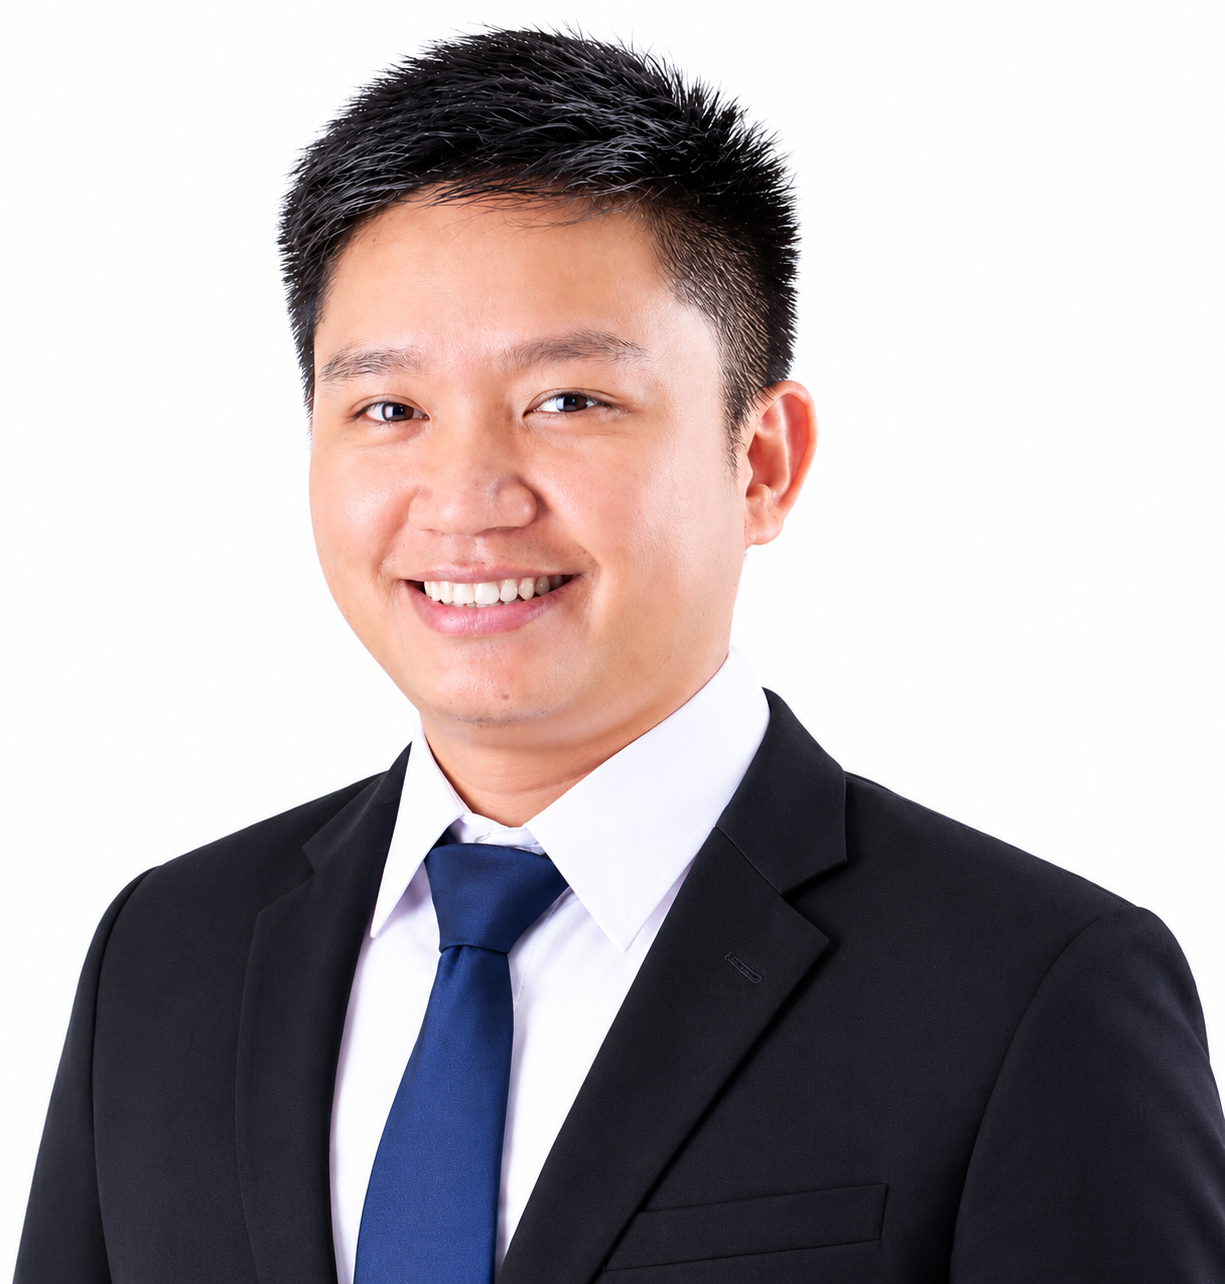
\includegraphics[width=1.5in,height=\textheight,keepaspectratio]{images/author/Bakti.png}

}

\caption{Foto Bakti Siregar, M.Sc.}

\end{figure}%

\textbf{\href{https://www.linkedin.com/in/dsciencelabs/}{Bakti Siregar,
M.Sc., CDS}} bekerja sebagai Dosen di Prodi Sains Data Institut
Teknologi Sains Bandung. Beliau adalah meraih gelar Magister-nya dari
Departemen Matematika Terapan (Applied Mathematics) National Sun Yat Sen
University, Taiwan. Selain mengajar beliau juga pernah bekerja sebagai
\textbf{Data Scientist Freelance} di perusahaan-perusahaan ternama
seperti \href{https://www.jne.co.id/id/beranda}{JNE},
\href{https://www.samoragroup.co.id/home/en}{Samora Group},
\href{https://www.pertamina.com/}{Pertamina}, dan saat ini masih aktif
sebagai \textbf{Data Scientist Freelance} di
\href{PT.\%20Green\%20City\%20Traffic}{PT. Green City Traffic}. Beliau
memiliki antusiasme khusus dalam mengerjakan proyek (mengajar) Big Data
Analytics, Machine Learning, Optimisasi, dan Analisis Time Series di
bidang keuangan dan investasi. Keahlian utama yang dimilikinya adalah
bahasa pemrograman Statistik seperti R Studio dan Python. Beliau juga
sudah terbiasa dalam mengaplikasikan sistem basis data MySQL/NoSQL untuk
manajemen data, serta mahir dalam menggunakan tools Big Data seperti
Spark dan Hadoop. Beberapa project beliau dapat dilihat di link berikut:
\href{https://rpubs.com/dsciencelabs}{Rpubs},
\href{https://github.com/dsciencelabs}{Github},
\href{https://dsciencelabs.github.io/web/index.html}{Website}, dan
\href{https://www.kaggle.com/baktisiregar/code}{Kaggle}.

\section*{Ucapan Terima Kasih}\label{ucapan-terima-kasih}
\addcontentsline{toc}{section}{Ucapan Terima Kasih}

\markright{Ucapan Terima Kasih}

Proses penulisan Tempate eBook ini tidak terlepas dari dukungan berbagai
pihak. Saya ingin mengucapkan terima kasih kepada:

\begin{itemize}
\tightlist
\item
  \textbf{Keluarga} yang selalu memberikan dukungan moral dan semangat
  tanpa henti.
\item
  \textbf{Rekan-rekan dan Kolaborator} yang telah memberikan masukan,
  saran, dan kritik yang konstruktif.
\item
  Institusi dan Organisasi, Khususnya
  \textbf{\href{https://itsb.ac.id/}{ITSB}} yang telah menyediakan
  sumber daya dan fasilitas yang diperlukan selama proses penelitian dan
  penulisan.
\end{itemize}

Saya berharap Template eBook ini dapat menjadi referensi yang bermanfaat
dan memberikan inspirasi serta pengetahuan baru bagi pembaca. Semoga
Ebook ini dapat memenuhi ekspektasi dan kebutuhan para pembaca dan
semoga ilmu yang disampaikan dapat bermanfaat bagi semua.

\section*{Masukan \& Saran}\label{masukan-saran}
\addcontentsline{toc}{section}{Masukan \& Saran}

\markright{Masukan \& Saran}

Semua masukan dan tanggapan Anda sangat berarti bagi kami untuk
memperbaiki Ebook Quarto Template ini kedepannya. Bagi para
pembaca/pengguna yang ingin menyampaikan masukan dan tanggapan,
dipersilahkan melalui kontak dibawah ini!

\textbf{Email:} dsciencelabs@outlook.com

\bookmarksetup{startatroot}

\chapter{Sampling Distribution}\label{sampling-distribution}

\section{Tiga Distribusi yang Harus
Dibedakan}\label{tiga-distribusi-yang-harus-dibedakan}

{\def\LTcaptype{none} % do not increment counter
\begin{longtable}[]{@{}
  >{\raggedright\arraybackslash}p{(\linewidth - 6\tabcolsep) * \real{0.2500}}
  >{\raggedright\arraybackslash}p{(\linewidth - 6\tabcolsep) * \real{0.2500}}
  >{\raggedright\arraybackslash}p{(\linewidth - 6\tabcolsep) * \real{0.2500}}
  >{\raggedright\arraybackslash}p{(\linewidth - 6\tabcolsep) * \real{0.2500}}@{}}
\toprule\noalign{}
\begin{minipage}[b]{\linewidth}\raggedright
Distribusi
\end{minipage} & \begin{minipage}[b]{\linewidth}\raggedright
Isinya
\end{minipage} & \begin{minipage}[b]{\linewidth}\raggedright
Jumlah nilai
\end{minipage} & \begin{minipage}[b]{\linewidth}\raggedright
Contoh
\end{minipage} \\
\midrule\noalign{}
\endhead
\bottomrule\noalign{}
\endlastfoot
\textbf{Distribusi populasi} & Nilai setiap unit populasi & \(N\) &
Pengeluaran 20.000 mahasiswa \\
\textbf{Distribusi sampel} & Nilai unit dalam satu sampel & \(n\) &
Pengeluaran 40 mahasiswa yang disurvei \\
\textbf{Distribusi sampling} & Nilai statistik (misalnya \(\bar{x}\))
dari banyak sampel & Sebanyak sampel yang (dibayangkan) diambil &
\(\bar{x}\) dari 10.000 sampel berukuran 40 \\
\end{longtable}
}

Distribusi sampling adalah konsep teoretis: dalam praktik kita hanya
memiliki satu sampel. Namun dengan simulasi kita dapat ``melihatnya''.

\subsection{Populasi Simulasi}\label{populasi-simulasi}

Kita memakai populasi 20.000 mahasiswa dengan variabel waktu layar
harian (jam) yang menjulur kanan --- bentuk yang sengaja dipilih jauh
dari lonceng.

\begin{Shaded}
\begin{Highlighting}[]
\FunctionTok{set.seed}\NormalTok{(}\DecValTok{909}\NormalTok{)}
\NormalTok{N }\OtherTok{\textless{}{-}} \DecValTok{20000}
\NormalTok{populasi }\OtherTok{\textless{}{-}} \FunctionTok{round}\NormalTok{(}\FunctionTok{rgamma}\NormalTok{(N, }\AttributeTok{shape =} \DecValTok{2}\NormalTok{, }\AttributeTok{rate =} \FloatTok{0.4}\NormalTok{), }\DecValTok{2}\NormalTok{) }\CommentTok{\# jam per hari}
\NormalTok{mu }\OtherTok{\textless{}{-}} \FunctionTok{mean}\NormalTok{(populasi)}
\NormalTok{sigma }\OtherTok{\textless{}{-}} \FunctionTok{sqrt}\NormalTok{(}\FunctionTok{mean}\NormalTok{((populasi }\SpecialCharTok{{-}}\NormalTok{ mu)}\SpecialCharTok{\^{}}\DecValTok{2}\NormalTok{)) }\CommentTok{\# SD populasi (pembagi N)}

\FunctionTok{c}\NormalTok{(}\AttributeTok{N =}\NormalTok{ N, }\AttributeTok{mu =} \FunctionTok{round}\NormalTok{(mu, }\DecValTok{3}\NormalTok{), }\AttributeTok{sigma =} \FunctionTok{round}\NormalTok{(sigma, }\DecValTok{3}\NormalTok{))}
\end{Highlighting}
\end{Shaded}

\begin{verbatim}
        N        mu     sigma 
20000.000     5.010     3.551 
\end{verbatim}

\begin{Shaded}
\begin{Highlighting}[]
\FunctionTok{set.seed}\NormalTok{(}\DecValTok{1}\NormalTok{)}
\NormalTok{satu\_sampel }\OtherTok{\textless{}{-}} \FunctionTok{sample}\NormalTok{(populasi, }\DecValTok{40}\NormalTok{)}
\NormalTok{banyak\_rata }\OtherTok{\textless{}{-}} \FunctionTok{replicate}\NormalTok{(}\DecValTok{10000}\NormalTok{, }\FunctionTok{mean}\NormalTok{(}\FunctionTok{sample}\NormalTok{(populasi, }\DecValTok{40}\NormalTok{)))}

\FunctionTok{par}\NormalTok{(}\AttributeTok{mfrow =} \FunctionTok{c}\NormalTok{(}\DecValTok{1}\NormalTok{, }\DecValTok{3}\NormalTok{))}
\FunctionTok{hist}\NormalTok{(populasi, }\AttributeTok{breaks =} \DecValTok{40}\NormalTok{, }\AttributeTok{col =} \StringTok{"\#9ecae1"}\NormalTok{, }\AttributeTok{border =} \StringTok{"white"}\NormalTok{,}
     \AttributeTok{main =} \StringTok{"Populasi (N = 20.000)"}\NormalTok{, }\AttributeTok{xlab =} \StringTok{"Jam per hari"}\NormalTok{, }\AttributeTok{xlim =} \FunctionTok{c}\NormalTok{(}\DecValTok{0}\NormalTok{, }\DecValTok{20}\NormalTok{))}
\FunctionTok{hist}\NormalTok{(satu\_sampel, }\AttributeTok{breaks =} \DecValTok{12}\NormalTok{, }\AttributeTok{col =} \StringTok{"\#fdae6b"}\NormalTok{, }\AttributeTok{border =} \StringTok{"white"}\NormalTok{,}
     \AttributeTok{main =} \StringTok{"Satu sampel (n = 40)"}\NormalTok{, }\AttributeTok{xlab =} \StringTok{"Jam per hari"}\NormalTok{, }\AttributeTok{xlim =} \FunctionTok{c}\NormalTok{(}\DecValTok{0}\NormalTok{, }\DecValTok{20}\NormalTok{))}
\FunctionTok{hist}\NormalTok{(banyak\_rata, }\AttributeTok{breaks =} \DecValTok{40}\NormalTok{, }\AttributeTok{col =} \StringTok{"\#a1d99b"}\NormalTok{, }\AttributeTok{border =} \StringTok{"white"}\NormalTok{,}
     \AttributeTok{main =} \StringTok{"Sampling distribution x{-}bar"}\NormalTok{, }\AttributeTok{xlab =} \StringTok{"Rata{-}rata sampel (n = 40)"}\NormalTok{)}
\end{Highlighting}
\end{Shaded}

\pandocbounded{\includegraphics[keepaspectratio]{chapters/bab-1_files/figure-pdf/unnamed-chunk-2-1.pdf}}

\begin{Shaded}
\begin{Highlighting}[]
\FunctionTok{par}\NormalTok{(}\AttributeTok{mfrow =} \FunctionTok{c}\NormalTok{(}\DecValTok{1}\NormalTok{, }\DecValTok{1}\NormalTok{))}
\end{Highlighting}
\end{Shaded}

Populasi dan satu sampel sama-sama menjulur kanan, tetapi distribusi
rata-rata sampel jauh lebih sempit dan hampir berbentuk lonceng. Inilah
inti pertemuan ini.

\section{Distribusi Sampling Rata-rata
Sampel}\label{distribusi-sampling-rata-rata-sampel}

Untuk sampel acak berukuran \(n\) dari populasi dengan mean \(\mu\) dan
simpangan baku \(\sigma\):

{\def\LTcaptype{none} % do not increment counter
\begin{longtable}[]{@{}
  >{\raggedright\arraybackslash}p{(\linewidth - 4\tabcolsep) * \real{0.3333}}
  >{\raggedright\arraybackslash}p{(\linewidth - 4\tabcolsep) * \real{0.3333}}
  >{\raggedright\arraybackslash}p{(\linewidth - 4\tabcolsep) * \real{0.3333}}@{}}
\toprule\noalign{}
\begin{minipage}[b]{\linewidth}\raggedright
Sifat
\end{minipage} & \begin{minipage}[b]{\linewidth}\raggedright
Rumus
\end{minipage} & \begin{minipage}[b]{\linewidth}\raggedright
Arti
\end{minipage} \\
\midrule\noalign{}
\endhead
\bottomrule\noalign{}
\endlastfoot
\textbf{Mean} & \(\mu_{\bar{x}} = \mu\) & \(\bar{x}\) adalah penaksir
tak bias: rata-ratanya tepat di parameter \\
\textbf{Standard error} & \(\sigma_{\bar{x}} = \frac{\sigma}{\sqrt{n}}\)
& Sebaran \(\bar{x}\) mengecil seiring bertambahnya \(n\) \\
\textbf{Bentuk} & Normal jika populasi normal; mendekati normal untuk
\(n\) cukup besar (CLT) & Memungkinkan perhitungan peluang \\
\end{longtable}
}

\begin{Shaded}
\begin{Highlighting}[]
\NormalTok{knitr}\SpecialCharTok{::}\FunctionTok{kable}\NormalTok{(}\FunctionTok{data.frame}\NormalTok{(}
  \AttributeTok{Besaran =} \FunctionTok{c}\NormalTok{(}\StringTok{"Mean distribusi sampling"}\NormalTok{, }\StringTok{"SD distribusi sampling (SE)"}\NormalTok{),}
  \AttributeTok{Teori =} \FunctionTok{round}\NormalTok{(}\FunctionTok{c}\NormalTok{(mu, sigma }\SpecialCharTok{/} \FunctionTok{sqrt}\NormalTok{(}\DecValTok{40}\NormalTok{)), }\DecValTok{4}\NormalTok{),}
  \AttributeTok{Simulasi\_10000\_sampel =} \FunctionTok{round}\NormalTok{(}\FunctionTok{c}\NormalTok{(}\FunctionTok{mean}\NormalTok{(banyak\_rata), }\FunctionTok{sd}\NormalTok{(banyak\_rata)), }\DecValTok{4}\NormalTok{)}
\NormalTok{), }\AttributeTok{caption =} \StringTok{"Teori vs simulasi untuk n = 40"}\NormalTok{)}
\end{Highlighting}
\end{Shaded}

\begin{longtable}[]{@{}lrr@{}}
\caption{Teori vs simulasi untuk n = 40}\tabularnewline
\toprule\noalign{}
Besaran & Teori & Simulasi\_10000\_sampel \\
\midrule\noalign{}
\endfirsthead
\toprule\noalign{}
Besaran & Teori & Simulasi\_10000\_sampel \\
\midrule\noalign{}
\endhead
\bottomrule\noalign{}
\endlastfoot
Mean distribusi sampling & 5.0097 & 5.0024 \\
SD distribusi sampling (SE) & 0.5615 & 0.5556 \\
\end{longtable}

Hasil simulasi hampir persis sama dengan teori.

\textbf{Koreksi populasi terhingga:} Rumus \(\sigma / \sqrt{n}\)
mengasumsikan populasi sangat besar dibanding sampel. Jika sampel
mencapai lebih dari sekitar 5\% populasi (tanpa pengembalian), \(SE\)
dikalikan faktor \(\sqrt{\frac{N - n}{N - 1}}\). Pada contoh ini
\(n/N = 0{,}2\%\) sehingga koreksi dapat diabaikan.

\subsection{Pengaruh Ukuran Sampel}\label{pengaruh-ukuran-sampel}

\begin{Shaded}
\begin{Highlighting}[]
\FunctionTok{set.seed}\NormalTok{(}\DecValTok{2}\NormalTok{)}
\NormalTok{n\_list }\OtherTok{\textless{}{-}} \FunctionTok{c}\NormalTok{(}\DecValTok{5}\NormalTok{, }\DecValTok{20}\NormalTok{, }\DecValTok{80}\NormalTok{)}

\FunctionTok{par}\NormalTok{(}\AttributeTok{mfrow =} \FunctionTok{c}\NormalTok{(}\DecValTok{1}\NormalTok{, }\DecValTok{3}\NormalTok{))}
\ControlFlowTok{for}\NormalTok{ (nn }\ControlFlowTok{in}\NormalTok{ n\_list) \{}
\NormalTok{  rata }\OtherTok{\textless{}{-}} \FunctionTok{replicate}\NormalTok{(}\DecValTok{5000}\NormalTok{, }\FunctionTok{mean}\NormalTok{(}\FunctionTok{sample}\NormalTok{(populasi, nn)))}
  \FunctionTok{hist}\NormalTok{(rata, }\AttributeTok{breaks =} \DecValTok{40}\NormalTok{, }\AttributeTok{col =} \StringTok{"\#a1d99b"}\NormalTok{, }\AttributeTok{border =} \StringTok{"white"}\NormalTok{, }\AttributeTok{xlim =} \FunctionTok{c}\NormalTok{(}\DecValTok{1}\NormalTok{, }\DecValTok{10}\NormalTok{),}
       \AttributeTok{freq =} \ConstantTok{FALSE}\NormalTok{,}
       \AttributeTok{main =} \FunctionTok{paste0}\NormalTok{(}\StringTok{"n = "}\NormalTok{, nn, }\StringTok{" (SE = "}\NormalTok{, }\FunctionTok{round}\NormalTok{(sigma }\SpecialCharTok{/} \FunctionTok{sqrt}\NormalTok{(nn), }\DecValTok{2}\NormalTok{), }\StringTok{")"}\NormalTok{),}
       \AttributeTok{xlab =} \StringTok{"Rata{-}rata sampel"}\NormalTok{)}
  \FunctionTok{curve}\NormalTok{(}\FunctionTok{dnorm}\NormalTok{(x, mu, sigma }\SpecialCharTok{/} \FunctionTok{sqrt}\NormalTok{(nn)), }\AttributeTok{add =} \ConstantTok{TRUE}\NormalTok{, }\AttributeTok{col =} \StringTok{"firebrick"}\NormalTok{, }\AttributeTok{lwd =} \DecValTok{2}\NormalTok{)}
  \FunctionTok{abline}\NormalTok{(}\AttributeTok{v =}\NormalTok{ mu, }\AttributeTok{lty =} \DecValTok{2}\NormalTok{)}
\NormalTok{\}}
\end{Highlighting}
\end{Shaded}

\pandocbounded{\includegraphics[keepaspectratio]{chapters/bab-1_files/figure-pdf/unnamed-chunk-5-1.pdf}}

\begin{Shaded}
\begin{Highlighting}[]
\FunctionTok{par}\NormalTok{(}\AttributeTok{mfrow =} \FunctionTok{c}\NormalTok{(}\DecValTok{1}\NormalTok{, }\DecValTok{1}\NormalTok{))}
\end{Highlighting}
\end{Shaded}

Kurva merah adalah distribusi normal dengan mean \(\mu\) dan SD
\(\sigma / \sqrt{n}\). Semakin besar \(n\):

\begin{enumerate}
\def\labelenumi{\arabic{enumi}.}
\tightlist
\item
  Distribusi semakin sempit.
\item
  Bentuknya semakin mendekati normal meskipun populasinya menjulur
  kanan.
\end{enumerate}

\section{Central Limit Theorem (CLT)}\label{central-limit-theorem-clt}

\textbf{Central Limit Theorem:} Jika sampel acak berukuran \(n\) diambil
dari populasi sembarang bentuk dengan mean \(\mu\) dan simpangan baku
\(\sigma\) (terhingga), maka untuk \(n\) yang cukup besar, distribusi
sampling \(\bar{x}\) mendekati normal:

\[\bar{x} \approx N\left(\mu, \frac{\sigma^2}{n}\right)\]

CLT adalah alasan mengapa distribusi normal muncul di mana-mana dalam
statistika inferensial --- bukan karena data selalu normal, tetapi
karena \textbf{rata-rata dari data cenderung normal}.

\subsection{Demonstrasi pada Tiga Bentuk
Populasi}\label{demonstrasi-pada-tiga-bentuk-populasi}

\begin{Shaded}
\begin{Highlighting}[]
\FunctionTok{set.seed}\NormalTok{(}\DecValTok{3}\NormalTok{)}
\NormalTok{pop\_bentuk }\OtherTok{\textless{}{-}} \FunctionTok{list}\NormalTok{(}
  \StringTok{"Seragam"} \OtherTok{=} \FunctionTok{runif}\NormalTok{(}\DecValTok{20000}\NormalTok{, }\DecValTok{0}\NormalTok{, }\DecValTok{10}\NormalTok{),}
  \StringTok{"Menjulur kanan"} \OtherTok{=} \FunctionTok{rexp}\NormalTok{(}\DecValTok{20000}\NormalTok{, }\AttributeTok{rate =} \FloatTok{0.5}\NormalTok{),}
  \StringTok{"Bimodal"} \OtherTok{=} \FunctionTok{c}\NormalTok{(}\FunctionTok{rnorm}\NormalTok{(}\DecValTok{10000}\NormalTok{, }\DecValTok{2}\NormalTok{, }\FloatTok{0.8}\NormalTok{), }\FunctionTok{rnorm}\NormalTok{(}\DecValTok{10000}\NormalTok{, }\DecValTok{8}\NormalTok{, }\FloatTok{0.8}\NormalTok{))}
\NormalTok{)}
\NormalTok{ukuran }\OtherTok{\textless{}{-}} \FunctionTok{c}\NormalTok{(}\DecValTok{2}\NormalTok{, }\DecValTok{5}\NormalTok{, }\DecValTok{30}\NormalTok{)}

\FunctionTok{par}\NormalTok{(}\AttributeTok{mfrow =} \FunctionTok{c}\NormalTok{(}\DecValTok{4}\NormalTok{, }\DecValTok{3}\NormalTok{), }\AttributeTok{mar =} \FunctionTok{c}\NormalTok{(}\DecValTok{3}\NormalTok{, }\DecValTok{3}\NormalTok{, }\FloatTok{2.5}\NormalTok{, }\DecValTok{1}\NormalTok{))}
\ControlFlowTok{for}\NormalTok{ (nama }\ControlFlowTok{in} \FunctionTok{names}\NormalTok{(pop\_bentuk)) \{}
  \FunctionTok{hist}\NormalTok{(pop\_bentuk[[nama]], }\AttributeTok{breaks =} \DecValTok{40}\NormalTok{, }\AttributeTok{col =} \StringTok{"\#9ecae1"}\NormalTok{, }\AttributeTok{border =} \StringTok{"white"}\NormalTok{,}
       \AttributeTok{main =} \FunctionTok{paste}\NormalTok{(}\StringTok{"Populasi:"}\NormalTok{, nama), }\AttributeTok{xlab =} \StringTok{""}\NormalTok{, }\AttributeTok{ylab =} \StringTok{""}\NormalTok{)}
\NormalTok{\}}
\ControlFlowTok{for}\NormalTok{ (nn }\ControlFlowTok{in}\NormalTok{ ukuran) \{}
  \ControlFlowTok{for}\NormalTok{ (nama }\ControlFlowTok{in} \FunctionTok{names}\NormalTok{(pop\_bentuk)) \{}
\NormalTok{    rata }\OtherTok{\textless{}{-}} \FunctionTok{replicate}\NormalTok{(}\DecValTok{3000}\NormalTok{, }\FunctionTok{mean}\NormalTok{(}\FunctionTok{sample}\NormalTok{(pop\_bentuk[[nama]], nn)))}
    \FunctionTok{hist}\NormalTok{(rata, }\AttributeTok{breaks =} \DecValTok{35}\NormalTok{, }\AttributeTok{col =} \StringTok{"\#a1d99b"}\NormalTok{, }\AttributeTok{border =} \StringTok{"white"}\NormalTok{,}
         \AttributeTok{main =} \FunctionTok{paste0}\NormalTok{(nama, }\StringTok{", n = "}\NormalTok{, nn), }\AttributeTok{xlab =} \StringTok{""}\NormalTok{, }\AttributeTok{ylab =} \StringTok{""}\NormalTok{)}
\NormalTok{  \}}
\NormalTok{\}}
\end{Highlighting}
\end{Shaded}

\pandocbounded{\includegraphics[keepaspectratio]{chapters/bab-1_files/figure-pdf/unnamed-chunk-7-1.pdf}}

\begin{Shaded}
\begin{Highlighting}[]
\FunctionTok{par}\NormalTok{(}\AttributeTok{mfrow =} \FunctionTok{c}\NormalTok{(}\DecValTok{1}\NormalTok{, }\DecValTok{1}\NormalTok{), }\AttributeTok{mar =} \FunctionTok{c}\NormalTok{(}\DecValTok{5}\NormalTok{, }\DecValTok{4}\NormalTok{, }\DecValTok{4}\NormalTok{, }\DecValTok{2}\NormalTok{) }\SpecialCharTok{+} \FloatTok{0.1}\NormalTok{)}
\end{Highlighting}
\end{Shaded}

Baris pertama adalah populasi; baris berikutnya adalah distribusi
sampling \(\bar{x}\) untuk \(n = 2\), \(5\), dan \(30\). Populasi
seragam sudah tampak lonceng pada \(n = 5\); populasi bimodal masih
bergelombang pada \(n = 2\) tetapi lonceng pada \(n = 30\); populasi
menjulur kanan membutuhkan \(n\) terbesar untuk menghilangkan
kemencengannya.

\subsection{Seberapa Besar ``Cukup
Besar''?}\label{seberapa-besar-cukup-besar}

{\def\LTcaptype{none} % do not increment counter
\begin{longtable}[]{@{}ll@{}}
\toprule\noalign{}
Bentuk populasi & Ukuran sampel yang biasanya cukup \\
\midrule\noalign{}
\endhead
\bottomrule\noalign{}
\endlastfoot
Normal & Berapa pun (distribusi \(\bar{x}\) tepat normal) \\
Simetris, tidak normal & Sekitar 10--15 \\
Menceng sedang & Sekitar 30 (aturan praktis yang populer) \\
Sangat menceng atau banyak outlier & Bisa jauh lebih dari 30 \\
\end{longtable}
}

\begin{Shaded}
\begin{Highlighting}[]
\NormalTok{skew }\OtherTok{\textless{}{-}} \ControlFlowTok{function}\NormalTok{(x) \{ d }\OtherTok{\textless{}{-}}\NormalTok{ x }\SpecialCharTok{{-}} \FunctionTok{mean}\NormalTok{(x); }\FunctionTok{mean}\NormalTok{(d}\SpecialCharTok{\^{}}\DecValTok{3}\NormalTok{) }\SpecialCharTok{/} \FunctionTok{mean}\NormalTok{(d}\SpecialCharTok{\^{}}\DecValTok{2}\NormalTok{)}\SpecialCharTok{\^{}}\FloatTok{1.5}\NormalTok{ \}}
\FunctionTok{set.seed}\NormalTok{(}\DecValTok{4}\NormalTok{)}
\FunctionTok{data.frame}\NormalTok{(}\AttributeTok{n =} \FunctionTok{c}\NormalTok{(}\DecValTok{2}\NormalTok{, }\DecValTok{5}\NormalTok{, }\DecValTok{10}\NormalTok{, }\DecValTok{30}\NormalTok{, }\DecValTok{100}\NormalTok{),}
\AttributeTok{Kemencengan\_xbar =} \FunctionTok{sapply}\NormalTok{(}\FunctionTok{c}\NormalTok{(}\DecValTok{2}\NormalTok{, }\DecValTok{5}\NormalTok{, }\DecValTok{10}\NormalTok{, }\DecValTok{30}\NormalTok{, }\DecValTok{100}\NormalTok{), }\ControlFlowTok{function}\NormalTok{(nn)}
\FunctionTok{round}\NormalTok{(}\FunctionTok{skew}\NormalTok{(}\FunctionTok{replicate}\NormalTok{(}\DecValTok{5000}\NormalTok{, }\FunctionTok{mean}\NormalTok{(}\FunctionTok{sample}\NormalTok{(populasi, nn)))), }\DecValTok{3}\NormalTok{)))}
\end{Highlighting}
\end{Shaded}

\begin{verbatim}
    n Kemencengan_xbar
1   2            1.007
2   5            0.581
3  10            0.470
4  30            0.220
5 100            0.170
\end{verbatim}

Kemencengan distribusi \(\bar{x}\) menyusut kira-kira sebanding dengan
\(1/\sqrt{n}\).

\subsection{Menghitung Peluang dengan
CLT}\label{menghitung-peluang-dengan-clt}

\textbf{Contoh:} Jika diambil sampel acak 40 mahasiswa, berapa peluang
rata-rata waktu layarnya melebihi \(5{,}5\) jam?

\[z = \frac{\bar{x} - \mu}{\sigma / \sqrt{n}}, \qquad P(\bar{x} > 5{,}5) = P(Z > z)\]

\begin{Shaded}
\begin{Highlighting}[]
\NormalTok{se40 }\OtherTok{\textless{}{-}}\NormalTok{ sigma }\SpecialCharTok{/} \FunctionTok{sqrt}\NormalTok{(}\DecValTok{40}\NormalTok{)}
\NormalTok{z\_55 }\OtherTok{\textless{}{-}}\NormalTok{ (}\FloatTok{5.5} \SpecialCharTok{{-}}\NormalTok{ mu) }\SpecialCharTok{/}\NormalTok{ se40}

\FunctionTok{c}\NormalTok{(}\AttributeTok{SE =} \FunctionTok{round}\NormalTok{(se40, }\DecValTok{4}\NormalTok{),}
  \AttributeTok{z =} \FunctionTok{round}\NormalTok{(z\_55, }\DecValTok{3}\NormalTok{),}
  \AttributeTok{Peluang\_CLT =} \FunctionTok{round}\NormalTok{(}\DecValTok{1} \SpecialCharTok{{-}} \FunctionTok{pnorm}\NormalTok{(z\_55), }\DecValTok{4}\NormalTok{),}
  \AttributeTok{Peluang\_simulasi =} \FunctionTok{round}\NormalTok{(}\FunctionTok{mean}\NormalTok{(banyak\_rata }\SpecialCharTok{\textgreater{}} \FloatTok{5.5}\NormalTok{), }\DecValTok{4}\NormalTok{))}
\end{Highlighting}
\end{Shaded}

\begin{verbatim}
              SE                z      Peluang_CLT Peluang_simulasi 
          0.5615           0.8730           0.1913           0.1803 
\end{verbatim}

Perbandingan: peluang \textbf{seorang mahasiswa} (bukan rata-rata 40
orang) memiliki waktu layar di atas \(5{,}5\) jam jauh lebih besar:

\begin{Shaded}
\begin{Highlighting}[]
\FunctionTok{mean}\NormalTok{(populasi }\SpecialCharTok{\textgreater{}} \FloatTok{5.5}\NormalTok{)}
\end{Highlighting}
\end{Shaded}

\begin{verbatim}
[1] 0.35175
\end{verbatim}

Individu sangat bervariasi, tetapi rata-rata dari banyak individu jauh
lebih stabil.

\section{Distribusi Sampling Proporsi
Sampel}\label{distribusi-sampling-proporsi-sampel}

Untuk variabel kategorik biner (Ya/Tidak), statistik yang dipakai adalah
proporsi sampel \(\hat{p} = x / n\).

{\def\LTcaptype{none} % do not increment counter
\begin{longtable}[]{@{}ll@{}}
\toprule\noalign{}
Sifat & Rumus \\
\midrule\noalign{}
\endhead
\bottomrule\noalign{}
\endlastfoot
\textbf{Mean} & \(\mu_{\hat{p}} = p\) \\
\textbf{Standard error} &
\(\sigma_{\hat{p}} = \sqrt{\frac{p(1 - p)}{n}}\) \\
\textbf{Bentuk} & Mendekati normal jika \(np \ge 10\) dan
\(n(1 - p) \ge 10\) \\
\end{longtable}
}

\begin{Shaded}
\begin{Highlighting}[]
\NormalTok{p\_benar }\OtherTok{\textless{}{-}} \FloatTok{0.08} \CommentTok{\# misalnya 8\% mahasiswa pernah terlambat membayar UKT}
\FunctionTok{set.seed}\NormalTok{(}\DecValTok{5}\NormalTok{)}

\FunctionTok{par}\NormalTok{(}\AttributeTok{mfrow =} \FunctionTok{c}\NormalTok{(}\DecValTok{1}\NormalTok{, }\DecValTok{3}\NormalTok{))}
\ControlFlowTok{for}\NormalTok{ (nn }\ControlFlowTok{in} \FunctionTok{c}\NormalTok{(}\DecValTok{20}\NormalTok{, }\DecValTok{60}\NormalTok{, }\DecValTok{300}\NormalTok{)) \{}
\NormalTok{  p\_hat }\OtherTok{\textless{}{-}} \FunctionTok{rbinom}\NormalTok{(}\DecValTok{5000}\NormalTok{, }\AttributeTok{size =}\NormalTok{ nn, }\AttributeTok{prob =}\NormalTok{ p\_benar) }\SpecialCharTok{/}\NormalTok{ nn}
  \FunctionTok{hist}\NormalTok{(p\_hat, }\AttributeTok{breaks =} \FunctionTok{seq}\NormalTok{(}\SpecialCharTok{{-}}\FloatTok{0.005}\NormalTok{, }\FloatTok{0.4}\NormalTok{, }\AttributeTok{by =} \FloatTok{0.01}\NormalTok{), }\AttributeTok{col =} \StringTok{"\#fdae6b"}\NormalTok{,}
       \AttributeTok{border =} \StringTok{"white"}\NormalTok{, }\AttributeTok{freq =} \ConstantTok{FALSE}\NormalTok{, }\AttributeTok{xlim =} \FunctionTok{c}\NormalTok{(}\DecValTok{0}\NormalTok{, }\FloatTok{0.3}\NormalTok{),}
       \AttributeTok{main =} \FunctionTok{paste0}\NormalTok{(}\StringTok{"n = "}\NormalTok{, nn, }\StringTok{": np = "}\NormalTok{, nn }\SpecialCharTok{*}\NormalTok{ p\_benar),}
       \AttributeTok{xlab =} \StringTok{"Proporsi sampel"}\NormalTok{)}
  \FunctionTok{curve}\NormalTok{(}\FunctionTok{dnorm}\NormalTok{(x, p\_benar, }\FunctionTok{sqrt}\NormalTok{(p\_benar }\SpecialCharTok{*}\NormalTok{ (}\DecValTok{1} \SpecialCharTok{{-}}\NormalTok{ p\_benar) }\SpecialCharTok{/}\NormalTok{ nn)),}
        \AttributeTok{add =} \ConstantTok{TRUE}\NormalTok{, }\AttributeTok{col =} \StringTok{"firebrick"}\NormalTok{, }\AttributeTok{lwd =} \DecValTok{2}\NormalTok{)}
\NormalTok{\}}
\end{Highlighting}
\end{Shaded}

\pandocbounded{\includegraphics[keepaspectratio]{chapters/bab-1_files/figure-pdf/unnamed-chunk-12-1.pdf}}

\begin{Shaded}
\begin{Highlighting}[]
\FunctionTok{par}\NormalTok{(}\AttributeTok{mfrow =} \FunctionTok{c}\NormalTok{(}\DecValTok{1}\NormalTok{, }\DecValTok{1}\NormalTok{))}
\end{Highlighting}
\end{Shaded}

Dengan \(n = 20\) (\(np = 1{,}6\)), distribusi \(\hat{p}\) sangat
menceng dan ``berbatang'' --- pendekatan normal buruk. Dengan
\(n = 300\) (\(np = 24\)), pendekatan normal sangat baik.

\section{Standard Error}\label{standard-error}

\subsection{Standard Error vs Simpangan
Baku}\label{standard-error-vs-simpangan-baku}

{\def\LTcaptype{none} % do not increment counter
\begin{longtable}[]{@{}
  >{\raggedright\arraybackslash}p{(\linewidth - 4\tabcolsep) * \real{0.3333}}
  >{\raggedright\arraybackslash}p{(\linewidth - 4\tabcolsep) * \real{0.3333}}
  >{\raggedright\arraybackslash}p{(\linewidth - 4\tabcolsep) * \real{0.3333}}@{}}
\toprule\noalign{}
\begin{minipage}[b]{\linewidth}\raggedright
Aspek
\end{minipage} & \begin{minipage}[b]{\linewidth}\raggedright
Simpangan baku (\(s\) atau \(\sigma\))
\end{minipage} & \begin{minipage}[b]{\linewidth}\raggedright
Standard error (\(SE\))
\end{minipage} \\
\midrule\noalign{}
\endhead
\bottomrule\noalign{}
\endlastfoot
\textbf{Mengukur sebaran} & Data individu & Statistik (misalnya
\(\bar{x}\)) dari sampel ke sampel \\
\textbf{Menjawab} & ``Seberapa beragam individu?'' & ``Seberapa tepat
taksiran kita?'' \\
\textbf{Jika \(n\) bertambah} & Tetap (mendekati \(\sigma\)) &
Mengecil \\
\textbf{Rumus (mean)} &
\(s = \sqrt{\frac{\sum(x_i - \bar{x})^2}{n - 1}}\) &
\(SE = \frac{s}{\sqrt{n}}\) \\
\end{longtable}
}

Karena \(\sigma\) biasanya tidak diketahui, \(SE\) ditaksir dengan
\(s/\sqrt{n}\) (untuk mean) atau \(\sqrt{\hat{p}(1 - \hat{p})/n}\)
(untuk proporsi).

\begin{Shaded}
\begin{Highlighting}[]
\FunctionTok{set.seed}\NormalTok{(}\DecValTok{6}\NormalTok{)}
\NormalTok{n\_besar }\OtherTok{\textless{}{-}} \FunctionTok{c}\NormalTok{(}\DecValTok{10}\NormalTok{, }\DecValTok{40}\NormalTok{, }\DecValTok{160}\NormalTok{, }\DecValTok{640}\NormalTok{)}

\NormalTok{knitr}\SpecialCharTok{::}\FunctionTok{kable}\NormalTok{(}\FunctionTok{t}\NormalTok{(}\FunctionTok{sapply}\NormalTok{(n\_besar, }\ControlFlowTok{function}\NormalTok{(nn) \{}
\NormalTok{  hasil }\OtherTok{\textless{}{-}} \FunctionTok{replicate}\NormalTok{(}\DecValTok{2000}\NormalTok{, \{}
\NormalTok{    s }\OtherTok{\textless{}{-}} \FunctionTok{sample}\NormalTok{(populasi, nn)}
    \FunctionTok{c}\NormalTok{(}\FunctionTok{sd}\NormalTok{(s), }\FunctionTok{sd}\NormalTok{(s) }\SpecialCharTok{/} \FunctionTok{sqrt}\NormalTok{(nn))}
\NormalTok{  \})}
  \FunctionTok{c}\NormalTok{(}\AttributeTok{n =}\NormalTok{ nn,}
    \AttributeTok{Rata\_SD\_sampel =} \FunctionTok{round}\NormalTok{(}\FunctionTok{mean}\NormalTok{(hasil[}\DecValTok{1}\NormalTok{, ]), }\DecValTok{3}\NormalTok{),}
    \AttributeTok{Rata\_SE\_taksiran =} \FunctionTok{round}\NormalTok{(}\FunctionTok{mean}\NormalTok{(hasil[}\DecValTok{2}\NormalTok{, ]), }\DecValTok{3}\NormalTok{))}
\NormalTok{\})), }\AttributeTok{caption =} \FunctionTok{paste0}\NormalTok{(}\StringTok{"Rata{-}rata dari 2.000 sampel per n: SD stabil di sekitar sigma = "}\NormalTok{,}
                      \FunctionTok{round}\NormalTok{(sigma, }\DecValTok{2}\NormalTok{), }\StringTok{", SE mengecil"}\NormalTok{))}
\end{Highlighting}
\end{Shaded}

\begin{longtable}[]{@{}rrr@{}}
\caption{Rata-rata dari 2.000 sampel per n: SD stabil di sekitar sigma =
3.55, SE mengecil}\tabularnewline
\toprule\noalign{}
n & Rata\_SD\_sampel & Rata\_SE\_taksiran \\
\midrule\noalign{}
\endfirsthead
\toprule\noalign{}
n & Rata\_SD\_sampel & Rata\_SE\_taksiran \\
\midrule\noalign{}
\endhead
\bottomrule\noalign{}
\endlastfoot
10 & 3.348 & 1.059 \\
40 & 3.493 & 0.552 \\
160 & 3.537 & 0.280 \\
640 & 3.551 & 0.140 \\
\end{longtable}

\subsection{Hukum Akar Kuadrat}\label{hukum-akar-kuadrat}

Karena \(SE \propto 1/\sqrt{n}\), untuk membagi dua \(SE\) dibutuhkan
sampel \textbf{empat kali lipat}. Presisi semakin mahal: menambah \(n\)
dari 100 ke 400 memberi keuntungan yang sama dengan dari 400 ke 1.600.

\begin{Shaded}
\begin{Highlighting}[]
\NormalTok{n\_seq }\OtherTok{\textless{}{-}} \DecValTok{10}\SpecialCharTok{:}\DecValTok{1000}
\FunctionTok{plot}\NormalTok{(n\_seq, sigma }\SpecialCharTok{/} \FunctionTok{sqrt}\NormalTok{(n\_seq), }\AttributeTok{type =} \StringTok{"l"}\NormalTok{, }\AttributeTok{lwd =} \DecValTok{2}\NormalTok{, }\AttributeTok{col =} \StringTok{"\#4C72B0"}\NormalTok{,}
     \AttributeTok{xlab =} \StringTok{"Ukuran sampel (n)"}\NormalTok{, }\AttributeTok{ylab =} \StringTok{"Standard error"}\NormalTok{,}
     \AttributeTok{main =} \StringTok{"SE Menurun Cepat di Awal, Lalu Melandai"}\NormalTok{)}
\FunctionTok{points}\NormalTok{(}\FunctionTok{c}\NormalTok{(}\DecValTok{100}\NormalTok{, }\DecValTok{400}\NormalTok{), sigma }\SpecialCharTok{/} \FunctionTok{sqrt}\NormalTok{(}\FunctionTok{c}\NormalTok{(}\DecValTok{100}\NormalTok{, }\DecValTok{400}\NormalTok{)), }\AttributeTok{pch =} \DecValTok{16}\NormalTok{, }\AttributeTok{col =} \StringTok{"firebrick"}\NormalTok{, }\AttributeTok{cex =} \FloatTok{1.3}\NormalTok{)}
\FunctionTok{text}\NormalTok{(}\FunctionTok{c}\NormalTok{(}\DecValTok{100}\NormalTok{, }\DecValTok{400}\NormalTok{), sigma }\SpecialCharTok{/} \FunctionTok{sqrt}\NormalTok{(}\FunctionTok{c}\NormalTok{(}\DecValTok{100}\NormalTok{, }\DecValTok{400}\NormalTok{)), }\AttributeTok{pos =} \DecValTok{3}\NormalTok{,}
     \AttributeTok{labels =} \FunctionTok{paste0}\NormalTok{(}\StringTok{"n = "}\NormalTok{, }\FunctionTok{c}\NormalTok{(}\DecValTok{100}\NormalTok{, }\DecValTok{400}\NormalTok{), }\StringTok{"}\SpecialCharTok{\textbackslash{}n}\StringTok{SE = "}\NormalTok{, }\FunctionTok{round}\NormalTok{(sigma }\SpecialCharTok{/} \FunctionTok{sqrt}\NormalTok{(}\FunctionTok{c}\NormalTok{(}\DecValTok{100}\NormalTok{, }\DecValTok{400}\NormalTok{)), }\DecValTok{2}\NormalTok{)))}
\end{Highlighting}
\end{Shaded}

\pandocbounded{\includegraphics[keepaspectratio]{chapters/bab-1_files/figure-pdf/unnamed-chunk-15-1.pdf}}

\section{Estimasi}\label{estimasi}

\subsection{Point Estimate}\label{point-estimate}

\emph{Point estimate} adalah satu angka yang menaksir parameter.

{\def\LTcaptype{none} % do not increment counter
\begin{longtable}[]{@{}lll@{}}
\toprule\noalign{}
Parameter & Point estimate & Penaksir tak bias? \\
\midrule\noalign{}
\endhead
\bottomrule\noalign{}
\endlastfoot
\(\mu\) & \(\bar{x}\) & Ya \\
\(p\) & \(\hat{p}\) & Ya \\
\(\sigma^2\) & \(s^2\) (pembagi \(n - 1\)) & Ya \\
\(\sigma\) & \(s\) & Sedikit bias (diabaikan dalam praktik) \\
\end{longtable}
}

Kelemahan \emph{point estimate}: hampir pasti tidak tepat sama dengan
parameter, dan tidak memberi tahu seberapa jauh melesetnya.

\subsection{Confidence Interval (Selang
Kepercayaan)}\label{confidence-interval-selang-kepercayaan}

Selang kepercayaan memberikan rentang nilai yang masuk akal bagi
parameter:

\[\text{Point estimate} \pm \underbrace{\text{nilai kritis} \times SE}_{\text{margin of error}}\]

\subsubsection{\texorpdfstring{CI untuk Mean, \(\sigma\) Diketahui
(\(z\))}{CI untuk Mean, \textbackslash sigma Diketahui (z)}}\label{ci-untuk-mean-sigma-diketahui-z}

\[\bar{x} \pm z_{\alpha/2} \frac{\sigma}{\sqrt{n}}\]

{\def\LTcaptype{none} % do not increment counter
\begin{longtable}[]{@{}lll@{}}
\toprule\noalign{}
Tingkat kepercayaan & \(\alpha\) & \(z_{\alpha/2}\) \\
\midrule\noalign{}
\endhead
\bottomrule\noalign{}
\endlastfoot
90\% & 0,10 & 1,645 \\
95\% & 0,05 & 1,960 \\
99\% & 0,01 & 2,576 \\
\end{longtable}
}

\begin{Shaded}
\begin{Highlighting}[]
\FunctionTok{round}\NormalTok{(}\FunctionTok{qnorm}\NormalTok{(}\FunctionTok{c}\NormalTok{(}\FloatTok{0.95}\NormalTok{, }\FloatTok{0.975}\NormalTok{, }\FloatTok{0.995}\NormalTok{)), }\DecValTok{3}\NormalTok{)}
\end{Highlighting}
\end{Shaded}

\begin{verbatim}
[1] 1.645 1.960 2.576
\end{verbatim}

\subsubsection{\texorpdfstring{CI untuk Mean, \(\sigma\) Tidak Diketahui
(\(t\))}{CI untuk Mean, \textbackslash sigma Tidak Diketahui (t)}}\label{ci-untuk-mean-sigma-tidak-diketahui-t}

Dalam praktik \(\sigma\) hampir tidak pernah diketahui dan diganti
\(s\). Penggantian ini menambah ketidakpastian, sehingga nilai kritis
diambil dari distribusi \(t\) dengan derajat bebas \(df = n - 1\):

\[\bar{x} \pm t_{\alpha/2,\, n-1} \frac{s}{\sqrt{n}}\]

\begin{Shaded}
\begin{Highlighting}[]
\FunctionTok{curve}\NormalTok{(}\FunctionTok{dnorm}\NormalTok{(x), }\SpecialCharTok{{-}}\DecValTok{4}\NormalTok{, }\DecValTok{4}\NormalTok{, }\AttributeTok{lwd =} \DecValTok{2}\NormalTok{, }\AttributeTok{ylab =} \StringTok{"Kepadatan"}\NormalTok{, }\AttributeTok{xlab =} \StringTok{"Nilai"}\NormalTok{,}
\AttributeTok{main =} \StringTok{"Distribusi t Berekor Lebih Tebal dari Normal"}\NormalTok{)}
\FunctionTok{curve}\NormalTok{(}\FunctionTok{dt}\NormalTok{(x, }\AttributeTok{df =} \DecValTok{3}\NormalTok{), }\AttributeTok{add =} \ConstantTok{TRUE}\NormalTok{, }\AttributeTok{lwd =} \DecValTok{2}\NormalTok{, }\AttributeTok{lty =} \DecValTok{2}\NormalTok{, }\AttributeTok{col =} \StringTok{"firebrick"}\NormalTok{)}
\FunctionTok{curve}\NormalTok{(}\FunctionTok{dt}\NormalTok{(x, }\AttributeTok{df =} \DecValTok{10}\NormalTok{), }\AttributeTok{add =} \ConstantTok{TRUE}\NormalTok{, }\AttributeTok{lwd =} \DecValTok{2}\NormalTok{, }\AttributeTok{lty =} \DecValTok{3}\NormalTok{, }\AttributeTok{col =} \StringTok{"darkorange"}\NormalTok{)}
\FunctionTok{legend}\NormalTok{(}\StringTok{"topright"}\NormalTok{, }\AttributeTok{bty =} \StringTok{"n"}\NormalTok{, }\AttributeTok{lwd =} \DecValTok{2}\NormalTok{, }\AttributeTok{lty =} \FunctionTok{c}\NormalTok{(}\DecValTok{1}\NormalTok{, }\DecValTok{2}\NormalTok{, }\DecValTok{3}\NormalTok{), }\AttributeTok{col =} \FunctionTok{c}\NormalTok{(}\StringTok{"black"}\NormalTok{, }\StringTok{"firebrick"}\NormalTok{, }\StringTok{"darkorange"}\NormalTok{),}
\AttributeTok{legend =} \FunctionTok{c}\NormalTok{(}\StringTok{"Normal baku (z)"}\NormalTok{, }\StringTok{"t, df = 3"}\NormalTok{, }\StringTok{"t, df = 10"}\NormalTok{))}
\end{Highlighting}
\end{Shaded}

\pandocbounded{\includegraphics[keepaspectratio]{chapters/bab-1_files/figure-pdf/unnamed-chunk-17-1.pdf}}

\begin{Shaded}
\begin{Highlighting}[]
\FunctionTok{data.frame}\NormalTok{(}\AttributeTok{df =} \FunctionTok{c}\NormalTok{(}\DecValTok{4}\NormalTok{, }\DecValTok{9}\NormalTok{, }\DecValTok{29}\NormalTok{, }\DecValTok{99}\NormalTok{, }\ConstantTok{Inf}\NormalTok{),}
\AttributeTok{t\_kritis\_95 =} \FunctionTok{round}\NormalTok{(}\FunctionTok{qt}\NormalTok{(}\FloatTok{0.975}\NormalTok{, }\AttributeTok{df =} \FunctionTok{c}\NormalTok{(}\DecValTok{4}\NormalTok{, }\DecValTok{9}\NormalTok{, }\DecValTok{29}\NormalTok{, }\DecValTok{99}\NormalTok{, }\ConstantTok{Inf}\NormalTok{)), }\DecValTok{3}\NormalTok{))}
\end{Highlighting}
\end{Shaded}

\begin{verbatim}
   df t_kritis_95
1   4       2.776
2   9       2.262
3  29       2.045
4  99       1.984
5 Inf       1.960
\end{verbatim}

Untuk sampel kecil, nilai kritis \(t\) lebih besar daripada \(1{,}96\)
(selang lebih lebar, ``hukuman'' karena menaksir \(\sigma\)). Saat \(n\)
membesar, distribusi \(t\) mendekati normal.

\subsubsection{Contoh Perhitungan}\label{contoh-perhitungan}

Satu sampel 40 mahasiswa (\texttt{satu\_sampel}) dipakai untuk menaksir
rata-rata waktu layar seluruh mahasiswa.

\begin{Shaded}
\begin{Highlighting}[]
\NormalTok{n1 }\OtherTok{\textless{}{-}} \FunctionTok{length}\NormalTok{(satu\_sampel)}
\NormalTok{xbar }\OtherTok{\textless{}{-}} \FunctionTok{mean}\NormalTok{(satu\_sampel)}
\NormalTok{s }\OtherTok{\textless{}{-}} \FunctionTok{sd}\NormalTok{(satu\_sampel)}
\NormalTok{t\_krit }\OtherTok{\textless{}{-}} \FunctionTok{qt}\NormalTok{(}\FloatTok{0.975}\NormalTok{, }\AttributeTok{df =}\NormalTok{ n1 }\SpecialCharTok{{-}} \DecValTok{1}\NormalTok{)}
\NormalTok{se\_hat }\OtherTok{\textless{}{-}}\NormalTok{ s }\SpecialCharTok{/} \FunctionTok{sqrt}\NormalTok{(n1)}
\NormalTok{moe }\OtherTok{\textless{}{-}}\NormalTok{ t\_krit }\SpecialCharTok{*}\NormalTok{ se\_hat}

\FunctionTok{c}\NormalTok{(}\AttributeTok{n =}\NormalTok{ n1,}
  \AttributeTok{x\_bar =} \FunctionTok{round}\NormalTok{(xbar, }\DecValTok{3}\NormalTok{),}
  \AttributeTok{s =} \FunctionTok{round}\NormalTok{(s, }\DecValTok{3}\NormalTok{),}
  \AttributeTok{SE =} \FunctionTok{round}\NormalTok{(se\_hat, }\DecValTok{3}\NormalTok{),}
  \AttributeTok{t\_kritis =} \FunctionTok{round}\NormalTok{(t\_krit, }\DecValTok{3}\NormalTok{),}
  \AttributeTok{MoE =} \FunctionTok{round}\NormalTok{(moe, }\DecValTok{3}\NormalTok{),}
  \AttributeTok{Bawah =} \FunctionTok{round}\NormalTok{(xbar }\SpecialCharTok{{-}}\NormalTok{ moe, }\DecValTok{3}\NormalTok{),}
  \AttributeTok{Atas =} \FunctionTok{round}\NormalTok{(xbar }\SpecialCharTok{+}\NormalTok{ moe, }\DecValTok{3}\NormalTok{))}
\end{Highlighting}
\end{Shaded}

\begin{verbatim}
       n    x_bar        s       SE t_kritis      MoE    Bawah     Atas 
  40.000    4.915    3.019    0.477    2.023    0.966    3.950    5.881 
\end{verbatim}

\begin{Shaded}
\begin{Highlighting}[]
\FunctionTok{t.test}\NormalTok{(satu\_sampel, }\AttributeTok{conf.level =} \FloatTok{0.95}\NormalTok{)}\SpecialCharTok{$}\NormalTok{conf.int }\CommentTok{\# fungsi bawaan R, hasil sama}
\end{Highlighting}
\end{Shaded}

\begin{verbatim}
[1] 3.949947 5.881053
attr(,"conf.level")
[1] 0.95
\end{verbatim}

\textbf{Laporan:} \emph{``Rata-rata waktu layar mahasiswa diperkirakan
\(4{,}92\) jam per hari, dengan selang kepercayaan 95\% antara
\(3{,}95\) dan \(5{,}88\) jam (\(n = 40\)).''}

\subsubsection{CI untuk Proporsi}\label{ci-untuk-proporsi}

\[\hat{p} \pm z_{\alpha/2} \sqrt{\frac{\hat{p}(1 - \hat{p})}{n}}, \qquad \text{syarat: } n\hat{p} \ge 10 \text{ dan } n(1 - \hat{p}) \ge 10\]

\begin{Shaded}
\begin{Highlighting}[]
\CommentTok{\# 138 dari 400 responden memakai QRIS setiap hari}
\NormalTok{x\_ya }\OtherTok{\textless{}{-}} \DecValTok{138}
\NormalTok{n\_resp }\OtherTok{\textless{}{-}} \DecValTok{400}
\NormalTok{p\_hat }\OtherTok{\textless{}{-}}\NormalTok{ x\_ya }\SpecialCharTok{/}\NormalTok{ n\_resp}
\NormalTok{se\_p }\OtherTok{\textless{}{-}} \FunctionTok{sqrt}\NormalTok{(p\_hat }\SpecialCharTok{*}\NormalTok{ (}\DecValTok{1} \SpecialCharTok{{-}}\NormalTok{ p\_hat) }\SpecialCharTok{/}\NormalTok{ n\_resp)}
\NormalTok{moe\_p }\OtherTok{\textless{}{-}} \FunctionTok{qnorm}\NormalTok{(}\FloatTok{0.975}\NormalTok{) }\SpecialCharTok{*}\NormalTok{ se\_p}

\FunctionTok{c}\NormalTok{(}\AttributeTok{p\_hat =}\NormalTok{ p\_hat,}
  \AttributeTok{SE =} \FunctionTok{round}\NormalTok{(se\_p, }\DecValTok{4}\NormalTok{),}
  \AttributeTok{MoE =} \FunctionTok{round}\NormalTok{(moe\_p, }\DecValTok{4}\NormalTok{),}
  \AttributeTok{Bawah =} \FunctionTok{round}\NormalTok{(p\_hat }\SpecialCharTok{{-}}\NormalTok{ moe\_p, }\DecValTok{4}\NormalTok{),}
  \AttributeTok{Atas =} \FunctionTok{round}\NormalTok{(p\_hat }\SpecialCharTok{+}\NormalTok{ moe\_p, }\DecValTok{4}\NormalTok{))}
\end{Highlighting}
\end{Shaded}

\begin{verbatim}
 p_hat     SE    MoE  Bawah   Atas 
0.3450 0.0238 0.0466 0.2984 0.3916 
\end{verbatim}

\begin{Shaded}
\begin{Highlighting}[]
\FunctionTok{c}\NormalTok{(}\AttributeTok{n\_p =}\NormalTok{ n\_resp }\SpecialCharTok{*}\NormalTok{ p\_hat, }\AttributeTok{n\_1\_min\_p =}\NormalTok{ n\_resp }\SpecialCharTok{*}\NormalTok{ (}\DecValTok{1} \SpecialCharTok{{-}}\NormalTok{ p\_hat)) }\CommentTok{\# syarat terpenuhi}
\end{Highlighting}
\end{Shaded}

\begin{verbatim}
      n_p n_1_min_p 
      138       262 
\end{verbatim}

\textbf{Laporan:} \emph{``Sekitar \(34{,}5\%\) responden memakai QRIS
setiap hari, margin of error \(\pm 4{,}7\) poin persentase (kepercayaan
95\%).''}

\subsection{Menafsirkan Selang Kepercayaan dengan
Benar}\label{menafsirkan-selang-kepercayaan-dengan-benar}

Kepercayaan 95\% adalah \textbf{sifat prosedurnya}, bukan satu selang
tertentu: jika pengambilan sampel dan perhitungan selang diulang
berkali-kali, sekitar 95\% selang yang dihasilkan akan memuat \(\mu\).

\begin{Shaded}
\begin{Highlighting}[]
\FunctionTok{set.seed}\NormalTok{(}\DecValTok{7}\NormalTok{)}
\NormalTok{B }\OtherTok{\textless{}{-}} \DecValTok{100}
\NormalTok{selang }\OtherTok{\textless{}{-}} \FunctionTok{t}\NormalTok{(}\FunctionTok{replicate}\NormalTok{(B, \{}
\NormalTok{  s\_i }\OtherTok{\textless{}{-}} \FunctionTok{sample}\NormalTok{(populasi, }\DecValTok{40}\NormalTok{)}
\NormalTok{  m }\OtherTok{\textless{}{-}} \FunctionTok{mean}\NormalTok{(s\_i)}
\NormalTok{  e }\OtherTok{\textless{}{-}} \FunctionTok{qt}\NormalTok{(}\FloatTok{0.975}\NormalTok{, }\DecValTok{39}\NormalTok{) }\SpecialCharTok{*} \FunctionTok{sd}\NormalTok{(s\_i) }\SpecialCharTok{/} \FunctionTok{sqrt}\NormalTok{(}\DecValTok{40}\NormalTok{)}
  \FunctionTok{c}\NormalTok{(}\AttributeTok{bawah =}\NormalTok{ m }\SpecialCharTok{{-}}\NormalTok{ e, }\AttributeTok{atas =}\NormalTok{ m }\SpecialCharTok{+}\NormalTok{ e)}
\NormalTok{\}))}
\NormalTok{memuat }\OtherTok{\textless{}{-}}\NormalTok{ selang[, }\StringTok{"bawah"}\NormalTok{] }\SpecialCharTok{\textless{}=}\NormalTok{ mu }\SpecialCharTok{\&}\NormalTok{ selang[, }\StringTok{"atas"}\NormalTok{] }\SpecialCharTok{\textgreater{}=}\NormalTok{ mu}

\FunctionTok{plot}\NormalTok{(}\ConstantTok{NULL}\NormalTok{, }\AttributeTok{xlim =} \FunctionTok{range}\NormalTok{(selang), }\AttributeTok{ylim =} \FunctionTok{c}\NormalTok{(}\DecValTok{1}\NormalTok{, B),}
     \AttributeTok{xlab =} \StringTok{"Waktu layar (jam)"}\NormalTok{, }\AttributeTok{ylab =} \StringTok{"Sampel ke{-}"}\NormalTok{,}
     \AttributeTok{main =} \FunctionTok{paste0}\NormalTok{(}\StringTok{"100 Selang Kepercayaan 95\%: "}\NormalTok{, }\FunctionTok{sum}\NormalTok{(memuat), }\StringTok{" memuat mu"}\NormalTok{))}
\FunctionTok{segments}\NormalTok{(selang[, }\StringTok{"bawah"}\NormalTok{], }\DecValTok{1}\SpecialCharTok{:}\NormalTok{B, selang[, }\StringTok{"atas"}\NormalTok{], }\DecValTok{1}\SpecialCharTok{:}\NormalTok{B,}
         \AttributeTok{col =} \FunctionTok{ifelse}\NormalTok{(memuat, }\StringTok{"grey50"}\NormalTok{, }\StringTok{"firebrick"}\NormalTok{),}
         \AttributeTok{lwd =} \FunctionTok{ifelse}\NormalTok{(memuat, }\DecValTok{1}\NormalTok{, }\FloatTok{2.5}\NormalTok{))}
\FunctionTok{abline}\NormalTok{(}\AttributeTok{v =}\NormalTok{ mu, }\AttributeTok{col =} \StringTok{"\#4C72B0"}\NormalTok{, }\AttributeTok{lwd =} \DecValTok{2}\NormalTok{)}
\end{Highlighting}
\end{Shaded}

\pandocbounded{\includegraphics[keepaspectratio]{chapters/bab-1_files/figure-pdf/unnamed-chunk-23-1.pdf}}

Garis merah adalah selang yang gagal memuat \(\mu\). Kita tidak pernah
tahu apakah selang kita termasuk yang merah, tetapi kita tahu
prosedurnya berhasil sekitar 95\% dari waktu.

{\def\LTcaptype{none} % do not increment counter
\begin{longtable}[]{@{}
  >{\raggedright\arraybackslash}p{(\linewidth - 4\tabcolsep) * \real{0.3333}}
  >{\raggedright\arraybackslash}p{(\linewidth - 4\tabcolsep) * \real{0.3333}}
  >{\raggedright\arraybackslash}p{(\linewidth - 4\tabcolsep) * \real{0.3333}}@{}}
\toprule\noalign{}
\begin{minipage}[b]{\linewidth}\raggedright
Tafsiran
\end{minipage} & \begin{minipage}[b]{\linewidth}\raggedright
Benar/Salah
\end{minipage} & \begin{minipage}[b]{\linewidth}\raggedright
Alasan
\end{minipage} \\
\midrule\noalign{}
\endhead
\bottomrule\noalign{}
\endlastfoot
``Kami 95\% yakin bahwa selang \(4{,}2\)--\(5{,}7\) jam memuat rata-rata
populasi.'' & \textbf{Benar} & Bahasa sehari-hari yang diterima \\
``95\% selang yang dibuat dengan prosedur ini akan memuat \(\mu\).'' &
\textbf{Benar} & Tafsiran paling tepat \\
``Ada peluang 95\% bahwa \(\mu\) berada di antara \(4{,}2\) dan
\(5{,}7\).'' & \textbf{Salah} & \(\mu\) bukan variabel acak; ia di dalam
atau di luar selang \\
``95\% mahasiswa memiliki waktu layar antara \(4{,}2\) dan \(5{,}7\)
jam.'' & \textbf{Salah} & CI adalah tentang rata-rata, bukan individu \\
``95\% rata-rata sampel lain akan jatuh di selang ini.'' &
\textbf{Salah} & CI menaksir parameter \(\mu\), bukan \(\bar{x}\) sampel
berikutnya \\
\end{longtable}
}

\subsection{Faktor yang Memengaruhi Lebar
Selang}\label{faktor-yang-memengaruhi-lebar-selang}

{\def\LTcaptype{none} % do not increment counter
\begin{longtable}[]{@{}
  >{\raggedright\arraybackslash}p{(\linewidth - 4\tabcolsep) * \real{0.3333}}
  >{\raggedright\arraybackslash}p{(\linewidth - 4\tabcolsep) * \real{0.3333}}
  >{\raggedright\arraybackslash}p{(\linewidth - 4\tabcolsep) * \real{0.3333}}@{}}
\toprule\noalign{}
\begin{minipage}[b]{\linewidth}\raggedright
Faktor
\end{minipage} & \begin{minipage}[b]{\linewidth}\raggedright
Jika dinaikkan
\end{minipage} & \begin{minipage}[b]{\linewidth}\raggedright
Dampak pada lebar selang
\end{minipage} \\
\midrule\noalign{}
\endhead
\bottomrule\noalign{}
\endlastfoot
Tingkat kepercayaan (\(90\% \rightarrow 99\%\)) & Nilai kritis naik &
\textbf{Melebar} \\
Ukuran sampel (\(n\)) & \(SE\) turun & \textbf{Menyempit} \\
Variabilitas data (\(s\)) & \(SE\) naik & \textbf{Melebar} \\
\end{longtable}
}

\begin{Shaded}
\begin{Highlighting}[]
\NormalTok{lebar }\OtherTok{\textless{}{-}} \ControlFlowTok{function}\NormalTok{(n, s, conf) \{}
  \DecValTok{2} \SpecialCharTok{*} \FunctionTok{qt}\NormalTok{(}\DecValTok{1} \SpecialCharTok{{-}}\NormalTok{ (}\DecValTok{1} \SpecialCharTok{{-}}\NormalTok{ conf) }\SpecialCharTok{/} \DecValTok{2}\NormalTok{, n }\SpecialCharTok{{-}} \DecValTok{1}\NormalTok{) }\SpecialCharTok{*}\NormalTok{ s }\SpecialCharTok{/} \FunctionTok{sqrt}\NormalTok{(n)}
\NormalTok{\}}

\NormalTok{tabel\_lebar }\OtherTok{\textless{}{-}} \FunctionTok{round}\NormalTok{(}\FunctionTok{outer}\NormalTok{(}\FunctionTok{c}\NormalTok{(}\DecValTok{20}\NormalTok{, }\DecValTok{80}\NormalTok{, }\DecValTok{320}\NormalTok{), }\FunctionTok{c}\NormalTok{(}\FloatTok{0.90}\NormalTok{, }\FloatTok{0.95}\NormalTok{, }\FloatTok{0.99}\NormalTok{),}
                           \FunctionTok{Vectorize}\NormalTok{(}\ControlFlowTok{function}\NormalTok{(n, cf) }\FunctionTok{lebar}\NormalTok{(n, }\AttributeTok{s =} \DecValTok{3}\NormalTok{, }\AttributeTok{conf =}\NormalTok{ cf))), }\DecValTok{3}\NormalTok{)}
\FunctionTok{dimnames}\NormalTok{(tabel\_lebar) }\OtherTok{\textless{}{-}} \FunctionTok{list}\NormalTok{(}\FunctionTok{c}\NormalTok{(}\StringTok{"n = 20"}\NormalTok{, }\StringTok{"n = 80"}\NormalTok{, }\StringTok{"n = 320"}\NormalTok{),}
                              \FunctionTok{c}\NormalTok{(}\StringTok{"90\%"}\NormalTok{, }\StringTok{"95\%"}\NormalTok{, }\StringTok{"99\%"}\NormalTok{))}
\NormalTok{knitr}\SpecialCharTok{::}\FunctionTok{kable}\NormalTok{(tabel\_lebar, }\AttributeTok{caption =} \StringTok{"Lebar CI (s = 3) menurut ukuran sampel dan tingkat kepercayaan"}\NormalTok{)}
\end{Highlighting}
\end{Shaded}

\begin{longtable}[]{@{}lrrr@{}}
\caption{Lebar CI (s = 3) menurut ukuran sampel dan tingkat
kepercayaan}\tabularnewline
\toprule\noalign{}
& 90\% & 95\% & 99\% \\
\midrule\noalign{}
\endfirsthead
\toprule\noalign{}
& 90\% & 95\% & 99\% \\
\midrule\noalign{}
\endhead
\bottomrule\noalign{}
\endlastfoot
n = 20 & 2.320 & 2.808 & 3.838 \\
n = 80 & 1.116 & 1.335 & 1.771 \\
n = 320 & 0.553 & 0.660 & 0.869 \\
\end{longtable}

\section{Menentukan Ukuran Sampel}\label{menentukan-ukuran-sampel}

Sebelum survei, peneliti biasanya menetapkan \emph{margin of error}
(\(E\)) yang diinginkan lalu menghitung \(n\) minimum (\textbf{selalu
dibulatkan ke atas}).

{\def\LTcaptype{none} % do not increment counter
\begin{longtable}[]{@{}
  >{\raggedright\arraybackslash}p{(\linewidth - 4\tabcolsep) * \real{0.3333}}
  >{\raggedright\arraybackslash}p{(\linewidth - 4\tabcolsep) * \real{0.3333}}
  >{\raggedright\arraybackslash}p{(\linewidth - 4\tabcolsep) * \real{0.3333}}@{}}
\toprule\noalign{}
\begin{minipage}[b]{\linewidth}\raggedright
Parameter
\end{minipage} & \begin{minipage}[b]{\linewidth}\raggedright
Rumus ukuran sampel
\end{minipage} & \begin{minipage}[b]{\linewidth}\raggedright
Keterangan
\end{minipage} \\
\midrule\noalign{}
\endhead
\bottomrule\noalign{}
\endlastfoot
\textbf{Mean} & \(n = \left(\frac{z_{\alpha/2}\sigma}{E}\right)^2\) &
\(\sigma\) ditaksir dari studi sebelumnya atau survei percontohan \\
\textbf{Proporsi} & \(n = \frac{z_{\alpha/2}^2 p(1 - p)}{E^2}\) & Jika
\(p\) tidak diketahui, pakai \(p = 0{,}5\) (paling konservatif) \\
\end{longtable}
}

\begin{Shaded}
\begin{Highlighting}[]
\NormalTok{n\_mean }\OtherTok{\textless{}{-}} \ControlFlowTok{function}\NormalTok{(sigma, E, }\AttributeTok{conf =} \FloatTok{0.95}\NormalTok{) }\FunctionTok{ceiling}\NormalTok{((}\FunctionTok{qnorm}\NormalTok{(}\DecValTok{1} \SpecialCharTok{{-}}\NormalTok{ (}\DecValTok{1} \SpecialCharTok{{-}}\NormalTok{ conf) }\SpecialCharTok{/} \DecValTok{2}\NormalTok{) }\SpecialCharTok{*}\NormalTok{ sigma }\SpecialCharTok{/}\NormalTok{ E)}\SpecialCharTok{\^{}}\DecValTok{2}\NormalTok{)}
\NormalTok{n\_prop }\OtherTok{\textless{}{-}} \ControlFlowTok{function}\NormalTok{(E, }\AttributeTok{p =} \FloatTok{0.5}\NormalTok{, }\AttributeTok{conf =} \FloatTok{0.95}\NormalTok{) }\FunctionTok{ceiling}\NormalTok{(}\FunctionTok{qnorm}\NormalTok{(}\DecValTok{1} \SpecialCharTok{{-}}\NormalTok{ (}\DecValTok{1} \SpecialCharTok{{-}}\NormalTok{ conf) }\SpecialCharTok{/} \DecValTok{2}\NormalTok{)}\SpecialCharTok{\^{}}\DecValTok{2} \SpecialCharTok{*}\NormalTok{ p }\SpecialCharTok{*}\NormalTok{ (}\DecValTok{1} \SpecialCharTok{{-}}\NormalTok{ p) }\SpecialCharTok{/}\NormalTok{ E}\SpecialCharTok{\^{}}\DecValTok{2}\NormalTok{)}
\FunctionTok{n\_mean}\NormalTok{(}\AttributeTok{sigma =} \FloatTok{3.5}\NormalTok{, }\AttributeTok{E =} \FloatTok{0.5}\NormalTok{) }\CommentTok{\# menaksir rata{-}rata waktu layar +{-} 0,5 jam}
\end{Highlighting}
\end{Shaded}

\begin{verbatim}
[1] 189
\end{verbatim}

\begin{Shaded}
\begin{Highlighting}[]
\NormalTok{knitr}\SpecialCharTok{::}\FunctionTok{kable}\NormalTok{(}\FunctionTok{data.frame}\NormalTok{(}\AttributeTok{MoE =} \FunctionTok{c}\NormalTok{(}\StringTok{"5\%"}\NormalTok{, }\StringTok{"3\%"}\NormalTok{, }\StringTok{"2\%"}\NormalTok{, }\StringTok{"1\%"}\NormalTok{),}
\AttributeTok{n\_minimum =} \FunctionTok{sapply}\NormalTok{(}\FunctionTok{c}\NormalTok{(}\FloatTok{0.05}\NormalTok{, }\FloatTok{0.03}\NormalTok{, }\FloatTok{0.02}\NormalTok{, }\FloatTok{0.01}\NormalTok{), n\_prop)),}
\AttributeTok{caption =} \StringTok{"Ukuran sampel survei proporsi (p = 0,5; kepercayaan 95\%)"}\NormalTok{)}
\end{Highlighting}
\end{Shaded}

\begin{longtable}[]{@{}lr@{}}
\caption{Ukuran sampel survei proporsi (p = 0,5; kepercayaan
95\%)}\tabularnewline
\toprule\noalign{}
MoE & n\_minimum \\
\midrule\noalign{}
\endfirsthead
\toprule\noalign{}
MoE & n\_minimum \\
\midrule\noalign{}
\endhead
\bottomrule\noalign{}
\endlastfoot
5\% & 385 \\
3\% & 1068 \\
2\% & 2401 \\
1\% & 9604 \\
\end{longtable}

Survei nasional dengan \emph{margin of error} sekitar \(\pm 3\%\)
memerlukan sekitar 1.000--1.100 responden, berapa pun ukuran populasinya
(asalkan populasi jauh lebih besar dari sampel). Memperkecil
\emph{margin of error} dari 2\% ke 1\% memerlukan sampel \textbf{empat
kali lipat}.

\begin{quote}
\textbf{Ukuran sampel tidak menyembuhkan bias.} Rumus di atas hanya
mengendalikan galat acak. Jika metode sampling bias (Pertemuan 3),
sampel sebesar apa pun tetap menghasilkan selang yang presisi di tempat
yang salah.
\end{quote}

\section{Studi Kasus Komprehensif: Survei Adopsi QRIS
UMKM}\label{studi-kasus-komprehensif-survei-adopsi-qris-umkm}

\textbf{Konteks:} Dinas Koperasi ingin menaksir (1) proporsi UMKM
kuliner yang menerima QRIS dan (2) rata-rata nilai transaksi QRIS harian
per UMKM pengguna. Survei acak sederhana terhadap 250 UMKM dari daftar
resmi menghasilkan data berikut.

\begin{Shaded}
\begin{Highlighting}[]
\FunctionTok{set.seed}\NormalTok{(}\DecValTok{2026}\NormalTok{)}
\NormalTok{n\_umkm }\OtherTok{\textless{}{-}} \DecValTok{250}
\NormalTok{terima\_qris }\OtherTok{\textless{}{-}} \FunctionTok{rbinom}\NormalTok{(n\_umkm, }\DecValTok{1}\NormalTok{, }\FloatTok{0.62}\NormalTok{)}
\NormalTok{nilai\_trx }\OtherTok{\textless{}{-}} \FunctionTok{round}\NormalTok{(}\FunctionTok{rlnorm}\NormalTok{(}\FunctionTok{sum}\NormalTok{(terima\_qris), }\AttributeTok{meanlog =} \FunctionTok{log}\NormalTok{(}\DecValTok{450000}\NormalTok{), }\AttributeTok{sdlog =} \FloatTok{0.6}\NormalTok{), }\SpecialCharTok{{-}}\DecValTok{3}\NormalTok{) }\CommentTok{\# Rp/hari}

\FunctionTok{c}\NormalTok{(}\AttributeTok{Jumlah\_pengguna =} \FunctionTok{sum}\NormalTok{(terima\_qris))}
\end{Highlighting}
\end{Shaded}

\begin{verbatim}
Jumlah_pengguna 
            165 
\end{verbatim}

\begin{Shaded}
\begin{Highlighting}[]
\FunctionTok{summary}\NormalTok{(nilai\_trx)}
\end{Highlighting}
\end{Shaded}

\begin{verbatim}
   Min. 1st Qu.  Median    Mean 3rd Qu.    Max. 
  98000  334000  472000  553685  653000 2192000 
\end{verbatim}

\subsection{Langkah 1: Estimasi
Proporsi}\label{langkah-1-estimasi-proporsi}

\begin{Shaded}
\begin{Highlighting}[]
\NormalTok{p\_hat\_u }\OtherTok{\textless{}{-}} \FunctionTok{mean}\NormalTok{(terima\_qris)}
\NormalTok{se\_u }\OtherTok{\textless{}{-}} \FunctionTok{sqrt}\NormalTok{(p\_hat\_u }\SpecialCharTok{*}\NormalTok{ (}\DecValTok{1} \SpecialCharTok{{-}}\NormalTok{ p\_hat\_u) }\SpecialCharTok{/}\NormalTok{ n\_umkm)}
\NormalTok{ci\_u }\OtherTok{\textless{}{-}}\NormalTok{ p\_hat\_u }\SpecialCharTok{+} \FunctionTok{c}\NormalTok{(}\SpecialCharTok{{-}}\DecValTok{1}\NormalTok{, }\DecValTok{1}\NormalTok{) }\SpecialCharTok{*} \FunctionTok{qnorm}\NormalTok{(}\FloatTok{0.975}\NormalTok{) }\SpecialCharTok{*}\NormalTok{ se\_u}

\FunctionTok{c}\NormalTok{(}\AttributeTok{n\_p =}\NormalTok{ n\_umkm }\SpecialCharTok{*}\NormalTok{ p\_hat\_u, }\AttributeTok{n\_1mp =}\NormalTok{ n\_umkm }\SpecialCharTok{*}\NormalTok{ (}\DecValTok{1} \SpecialCharTok{{-}}\NormalTok{ p\_hat\_u)) }\CommentTok{\# cek syarat}
\end{Highlighting}
\end{Shaded}

\begin{verbatim}
  n_p n_1mp 
  165    85 
\end{verbatim}

\begin{Shaded}
\begin{Highlighting}[]
\FunctionTok{round}\NormalTok{(}\FunctionTok{c}\NormalTok{(}\AttributeTok{p\_hat =}\NormalTok{ p\_hat\_u, }\AttributeTok{SE =}\NormalTok{ se\_u, }\AttributeTok{Bawah =}\NormalTok{ ci\_u[}\DecValTok{1}\NormalTok{], }\AttributeTok{Atas =}\NormalTok{ ci\_u[}\DecValTok{2}\NormalTok{]), }\DecValTok{4}\NormalTok{)}
\end{Highlighting}
\end{Shaded}

\begin{verbatim}
 p_hat     SE  Bawah   Atas 
0.6600 0.0300 0.6013 0.7187 
\end{verbatim}

\subsection{Langkah 2: Estimasi Rata-rata Nilai
Transaksi}\label{langkah-2-estimasi-rata-rata-nilai-transaksi}

\begin{Shaded}
\begin{Highlighting}[]
\FunctionTok{hist}\NormalTok{(nilai\_trx }\SpecialCharTok{/} \DecValTok{1000}\NormalTok{, }\AttributeTok{breaks =} \DecValTok{25}\NormalTok{, }\AttributeTok{col =} \StringTok{"\#4C72B0"}\NormalTok{, }\AttributeTok{border =} \StringTok{"white"}\NormalTok{,}
     \AttributeTok{main =} \StringTok{"Nilai Transaksi QRIS Harian (UMKM pengguna)"}\NormalTok{,}
     \AttributeTok{xlab =} \StringTok{"Ribu Rp per hari"}\NormalTok{, }\AttributeTok{ylab =} \StringTok{"Jumlah UMKM"}\NormalTok{)}
\end{Highlighting}
\end{Shaded}

\pandocbounded{\includegraphics[keepaspectratio]{chapters/bab-1_files/figure-pdf/unnamed-chunk-30-1.pdf}}

\begin{Shaded}
\begin{Highlighting}[]
\NormalTok{ci\_trx }\OtherTok{\textless{}{-}} \FunctionTok{t.test}\NormalTok{(nilai\_trx)}\SpecialCharTok{$}\NormalTok{conf.int}
\FunctionTok{round}\NormalTok{(}\FunctionTok{c}\NormalTok{(}\AttributeTok{n =} \FunctionTok{length}\NormalTok{(nilai\_trx),}
        \AttributeTok{Mean =} \FunctionTok{mean}\NormalTok{(nilai\_trx),}
        \AttributeTok{Median =} \FunctionTok{median}\NormalTok{(nilai\_trx),}
        \AttributeTok{SE =} \FunctionTok{sd}\NormalTok{(nilai\_trx) }\SpecialCharTok{/} \FunctionTok{sqrt}\NormalTok{(}\FunctionTok{length}\NormalTok{(nilai\_trx)),}
        \AttributeTok{Bawah =}\NormalTok{ ci\_trx[}\DecValTok{1}\NormalTok{],}
        \AttributeTok{Atas =}\NormalTok{ ci\_trx[}\DecValTok{2}\NormalTok{]))}
\end{Highlighting}
\end{Shaded}

\begin{verbatim}
     n   Mean Median     SE  Bawah   Atas 
   165 553685 472000  24623 505065 602304 
\end{verbatim}

\subsection{Langkah 3: Apakah CLT Dapat Diandalkan di
Sini?}\label{langkah-3-apakah-clt-dapat-diandalkan-di-sini}

Datanya menjulur kanan. Kita periksa dengan \textbf{bootstrap}:
mengambil ulang sampel (dengan pengembalian) dari data kita sendiri
untuk meniru distribusi sampling \(\bar{x}\).

\begin{Shaded}
\begin{Highlighting}[]
\FunctionTok{set.seed}\NormalTok{(}\DecValTok{11}\NormalTok{)}
\NormalTok{boot\_mean }\OtherTok{\textless{}{-}} \FunctionTok{replicate}\NormalTok{(}\DecValTok{5000}\NormalTok{, }\FunctionTok{mean}\NormalTok{(}\FunctionTok{sample}\NormalTok{(nilai\_trx, }\AttributeTok{replace =} \ConstantTok{TRUE}\NormalTok{)))}

\FunctionTok{hist}\NormalTok{(boot\_mean }\SpecialCharTok{/} \DecValTok{1000}\NormalTok{, }\AttributeTok{breaks =} \DecValTok{40}\NormalTok{, }\AttributeTok{col =} \StringTok{"\#a1d99b"}\NormalTok{, }\AttributeTok{border =} \StringTok{"white"}\NormalTok{, }\AttributeTok{freq =} \ConstantTok{FALSE}\NormalTok{,}
     \AttributeTok{main =} \StringTok{"Distribusi Bootstrap Rata{-}rata Nilai Transaksi"}\NormalTok{,}
     \AttributeTok{xlab =} \StringTok{"Ribu Rp per hari"}\NormalTok{)}
\FunctionTok{curve}\NormalTok{(}\FunctionTok{dnorm}\NormalTok{(x, }\FunctionTok{mean}\NormalTok{(nilai\_trx) }\SpecialCharTok{/} \DecValTok{1000}\NormalTok{, }\FunctionTok{sd}\NormalTok{(nilai\_trx) }\SpecialCharTok{/} \FunctionTok{sqrt}\NormalTok{(}\FunctionTok{length}\NormalTok{(nilai\_trx)) }\SpecialCharTok{/} \DecValTok{1000}\NormalTok{),}
      \AttributeTok{add =} \ConstantTok{TRUE}\NormalTok{, }\AttributeTok{col =} \StringTok{"firebrick"}\NormalTok{, }\AttributeTok{lwd =} \DecValTok{2}\NormalTok{)}
\end{Highlighting}
\end{Shaded}

\pandocbounded{\includegraphics[keepaspectratio]{chapters/bab-1_files/figure-pdf/unnamed-chunk-32-1.pdf}}

\begin{Shaded}
\begin{Highlighting}[]
\FunctionTok{round}\NormalTok{(}\FunctionTok{quantile}\NormalTok{(boot\_mean, }\FunctionTok{c}\NormalTok{(}\FloatTok{0.025}\NormalTok{, }\FloatTok{0.975}\NormalTok{))) }\CommentTok{\# selang bootstrap persentil 95\%}
\end{Highlighting}
\end{Shaded}

\begin{verbatim}
  2.5%  97.5% 
506082 605874 
\end{verbatim}

Distribusi bootstrap hampir berbentuk lonceng dan selang bootstrap
hampir sama dengan selang \(t\). Dengan \(n = 165\) pengguna, CLT
bekerja baik meskipun data individunya menceng.

\subsection{Langkah 4: Merencanakan Survei
Lanjutan}\label{langkah-4-merencanakan-survei-lanjutan}

Dinas ingin survei tahun depan menghasilkan \emph{margin of error}
proporsi \(\pm 3\%\) dan rata-rata transaksi \(\pm \text{Rp } 30.000\)
(kepercayaan 95\%).

\begin{Shaded}
\begin{Highlighting}[]
\FunctionTok{c}\NormalTok{(}\AttributeTok{n\_untuk\_proporsi =} \FunctionTok{n\_prop}\NormalTok{(}\AttributeTok{E =} \FloatTok{0.03}\NormalTok{, }\AttributeTok{p =}\NormalTok{ p\_hat\_u),}
  \AttributeTok{n\_pengguna\_untuk\_mean =} \FunctionTok{n\_mean}\NormalTok{(}\AttributeTok{sigma =} \FunctionTok{sd}\NormalTok{(nilai\_trx), }\AttributeTok{E =} \DecValTok{30000}\NormalTok{))}
\end{Highlighting}
\end{Shaded}

\begin{verbatim}
     n_untuk_proporsi n_pengguna_untuk_mean 
                  958                   427 
\end{verbatim}

\subsection{Pertanyaan Diskusi dan
Jawaban}\label{pertanyaan-diskusi-dan-jawaban}

\begin{enumerate}
\def\labelenumi{\arabic{enumi}.}
\tightlist
\item
  \textbf{Bagaimana melaporkan hasil proporsi?} \emph{``Diperkirakan
  66\% UMKM kuliner telah menerima QRIS (CI 95\%: 60,1\%--71,9\%;
  \(n = 250\)).''} Kalimat ini memuat \emph{point estimate}, selang,
  tingkat kepercayaan, dan ukuran sampel.
\item
  \textbf{Mengapa median transaksi jauh di bawah mean, dan mana yang
  dilaporkan?} Distribusinya menjulur kanan (segelintir UMKM besar).
  Untuk menggambarkan UMKM tipikal, \textbf{median} lebih tepat. Namun
  jika dinas ingin menaksir total nilai transaksi
  (\(\text{mean} \times \text{jumlah UMKM pengguna}\)), yang dibutuhkan
  justru \textbf{mean} beserta selangnya.
\item
  \textbf{Apakah selang 95\% berarti 95\% UMKM bertransaksi di rentang
  tersebut?} \textbf{Tidak.} Selang itu menaksir rata-rata populasi.
  Rentang nilai transaksi individu jauh lebih lebar (lihat histogram).
\item
  \textbf{Mengapa ukuran sampel untuk proporsi tidak dihitung dengan
  \(p = 0{,}5\)?} Kita sudah memiliki taksiran
  \(\hat{p} \approx 0{,}66\) dari survei ini. Memakai \(p = 0{,}5\)
  lebih aman (menghasilkan \(n\) terbesar), tetapi dengan informasi
  sebelumnya kita dapat menghemat biaya. Perbedaannya kecil karena
  \(p(1 - p)\) hampir datar di sekitar \(0{,}5\).
\end{enumerate}

\section{Latihan Mandiri}\label{latihan-mandiri}

\subsection{Latihan Utama: Berat Kemasan Kopi
Bubuk}\label{latihan-utama-berat-kemasan-kopi-bubuk}

\textbf{Konteks:} Mesin pengisi kopi bubuk dirancang mengisi kemasan
dengan rata-rata \(250\) gram. Dari data historis, simpangan baku
pengisian \(\sigma = 6\) gram. Petugas QC mengambil sampel acak \(36\)
kemasan.

\begin{Shaded}
\begin{Highlighting}[]
\FunctionTok{set.seed}\NormalTok{(}\DecValTok{99}\NormalTok{)}
\NormalTok{berat }\OtherTok{\textless{}{-}} \FunctionTok{round}\NormalTok{(}\FunctionTok{rnorm}\NormalTok{(}\DecValTok{36}\NormalTok{, }\AttributeTok{mean =} \FloatTok{248.5}\NormalTok{, }\AttributeTok{sd =} \DecValTok{6}\NormalTok{), }\DecValTok{1}\NormalTok{)}
\FunctionTok{summary}\NormalTok{(berat)}
\end{Highlighting}
\end{Shaded}

\begin{verbatim}
   Min. 1st Qu.  Median    Mean 3rd Qu.    Max. 
  230.3   244.9   249.1   247.4   251.4   256.9 
\end{verbatim}

\subsubsection{Tugas 1: Hitung SE dan jelaskan
maknanya}\label{tugas-1-hitung-se-dan-jelaskan-maknanya}

\begin{Shaded}
\begin{Highlighting}[]
\NormalTok{sigma\_k }\OtherTok{\textless{}{-}} \DecValTok{6}
\NormalTok{n\_k }\OtherTok{\textless{}{-}} \FunctionTok{length}\NormalTok{(berat)}
\NormalTok{se\_k }\OtherTok{\textless{}{-}}\NormalTok{ sigma\_k }\SpecialCharTok{/} \FunctionTok{sqrt}\NormalTok{(n\_k)}
\NormalTok{se\_k}
\end{Highlighting}
\end{Shaded}

\begin{verbatim}
[1] 1
\end{verbatim}

\textbf{Jawaban:} \(SE = 6 / \sqrt{36} = 1\) gram. Rata-rata dari 36
kemasan biasanya meleset sekitar 1 gram dari rata-rata sebenarnya ---
jauh lebih kecil daripada variasi berat antarkemasan (6 gram).

\subsubsection{\texorpdfstring{Tugas 2: Jika mesin bekerja benar
(\(\mu = 250\)), berapa peluang rata-rata 36 kemasan kurang dari 248
gram?}{Tugas 2: Jika mesin bekerja benar (\textbackslash mu = 250), berapa peluang rata-rata 36 kemasan kurang dari 248 gram?}}\label{tugas-2-jika-mesin-bekerja-benar-mu-250-berapa-peluang-rata-rata-36-kemasan-kurang-dari-248-gram}

\begin{Shaded}
\begin{Highlighting}[]
\FunctionTok{pnorm}\NormalTok{(}\DecValTok{248}\NormalTok{, }\AttributeTok{mean =} \DecValTok{250}\NormalTok{, }\AttributeTok{sd =}\NormalTok{ sigma\_k }\SpecialCharTok{/} \FunctionTok{sqrt}\NormalTok{(n\_k))}
\end{Highlighting}
\end{Shaded}

\begin{verbatim}
[1] 0.02275013
\end{verbatim}

\textbf{Jawaban:} \(z = (248 - 250) / 1 = -2\) sehingga peluangnya
sekitar \textbf{\(0{,}0228\)} (\(2{,}28\%\)). Kejadian ini jarang jika
mesin bekerja benar --- gagasan yang menjadi dasar uji hipotesis di
Pertemuan 10.

\subsubsection{\texorpdfstring{Tugas 3: Hitung CI 95\% untuk rata-rata
berat (\(\sigma\)
diketahui)}{Tugas 3: Hitung CI 95\% untuk rata-rata berat (\textbackslash sigma diketahui)}}\label{tugas-3-hitung-ci-95-untuk-rata-rata-berat-sigma-diketahui}

\begin{Shaded}
\begin{Highlighting}[]
\NormalTok{ci\_z }\OtherTok{\textless{}{-}} \FunctionTok{mean}\NormalTok{(berat) }\SpecialCharTok{+} \FunctionTok{c}\NormalTok{(}\SpecialCharTok{{-}}\DecValTok{1}\NormalTok{, }\DecValTok{1}\NormalTok{) }\SpecialCharTok{*} \FunctionTok{qnorm}\NormalTok{(}\FloatTok{0.975}\NormalTok{) }\SpecialCharTok{*}\NormalTok{ sigma\_k }\SpecialCharTok{/} \FunctionTok{sqrt}\NormalTok{(n\_k)}
\FunctionTok{round}\NormalTok{(}\FunctionTok{c}\NormalTok{(}\AttributeTok{x\_bar =} \FunctionTok{mean}\NormalTok{(berat), }\AttributeTok{Bawah =}\NormalTok{ ci\_z[}\DecValTok{1}\NormalTok{], }\AttributeTok{Atas =}\NormalTok{ ci\_z[}\DecValTok{2}\NormalTok{]), }\DecValTok{2}\NormalTok{)}
\end{Highlighting}
\end{Shaded}

\begin{verbatim}
 x_bar  Bawah   Atas 
247.40 245.44 249.36 
\end{verbatim}

\subsubsection{\texorpdfstring{Tugas 4: Hitung CI 95\% jika \(\sigma\)
dianggap tidak diketahui
(\(t\))}{Tugas 4: Hitung CI 95\% jika \textbackslash sigma dianggap tidak diketahui (t)}}\label{tugas-4-hitung-ci-95-jika-sigma-dianggap-tidak-diketahui-t}

\begin{Shaded}
\begin{Highlighting}[]
\FunctionTok{round}\NormalTok{(}\FunctionTok{t.test}\NormalTok{(berat)}\SpecialCharTok{$}\NormalTok{conf.int, }\DecValTok{2}\NormalTok{)}
\end{Highlighting}
\end{Shaded}

\begin{verbatim}
[1] 245.25 249.56
attr(,"conf.level")
[1] 0.95
\end{verbatim}

\begin{Shaded}
\begin{Highlighting}[]
\FunctionTok{round}\NormalTok{(}\FunctionTok{c}\NormalTok{(}\AttributeTok{s =} \FunctionTok{sd}\NormalTok{(berat), }\AttributeTok{t\_kritis =} \FunctionTok{qt}\NormalTok{(}\FloatTok{0.975}\NormalTok{, }\DecValTok{35}\NormalTok{), }\AttributeTok{z\_kritis =} \FunctionTok{qnorm}\NormalTok{(}\FloatTok{0.975}\NormalTok{)), }\DecValTok{3}\NormalTok{)}
\end{Highlighting}
\end{Shaded}

\begin{verbatim}
       s t_kritis z_kritis 
   6.366    2.030    1.960 
\end{verbatim}

\subsubsection{Tugas 5: Tafsirkan
hasilnya}\label{tugas-5-tafsirkan-hasilnya}

\textbf{Jawaban:} Selang \(z\) (\([245{,}44;\ 249{,}36]\)) dan selang
\(t\) (\([245{,}25;\ 249{,}56]\)) sangat mirip karena \(n = 36\) cukup
besar (\(t\) kritis hanya sedikit di atas \(1{,}96\)) dan
\(s = 6{,}366\) dekat dengan \(\sigma = 6\). Karena nilai target \(250\)
gram berada di luar selang kepercayaan 95\%, data memberi indikasi bahwa
rata-rata pengisian mesin berbeda dari target --- yang dapat
dikonfirmasi dengan uji hipotesis.

\subsubsection{Tugas 6 (Tantangan): Ukuran
sampel}\label{tugas-6-tantangan-ukuran-sampel}

Berapa kemasan yang harus diambil agar \emph{margin of error} CI 95\%
hanya \(\pm 1\) gram? Dan \(\pm 0{,}5\) gram?

\begin{Shaded}
\begin{Highlighting}[]
\FunctionTok{c}\NormalTok{(}\AttributeTok{MoE\_1 =} \FunctionTok{n\_mean}\NormalTok{(}\AttributeTok{sigma =} \DecValTok{6}\NormalTok{, }\AttributeTok{E =} \DecValTok{1}\NormalTok{),}
  \AttributeTok{MoE\_0.5 =} \FunctionTok{n\_mean}\NormalTok{(}\AttributeTok{sigma =} \DecValTok{6}\NormalTok{, }\AttributeTok{E =} \FloatTok{0.5}\NormalTok{))}
\end{Highlighting}
\end{Shaded}

\begin{verbatim}
  MoE_1 MoE_0.5 
    139     554 
\end{verbatim}

\textbf{Jawaban:} \textbf{139 kemasan} untuk \(\pm 1\) gram dan
\textbf{554 kemasan} untuk \(\pm 0{,}5\) gram --- membagi dua
\emph{margin of error} membutuhkan sampel empat kali lipat.

\subsection{Latihan Tambahan
(Self-Check)}\label{latihan-tambahan-self-check}

\subsubsection{Soal A: Waktu Tunggu Layanan
Pelanggan}\label{soal-a-waktu-tunggu-layanan-pelanggan}

Waktu tunggu layanan pelanggan berdistribusi menjulur kanan dengan
\(\mu = 8\) menit dan \(\sigma = 6\) menit. Untuk sampel acak \(64\)
panggilan, tentukan mean, \(SE\), dan bentuk distribusi sampling
\(\bar{x}\), lalu hitung \(P(\bar{x} > 9)\).

\begin{Shaded}
\begin{Highlighting}[]
\CommentTok{\# Kunci jawaban:}
\CommentTok{\# Mean = 8; SE = 6 / sqrt(64) = 0.75; bentuk mendekati normal (CLT, n = 64)}
\DecValTok{1} \SpecialCharTok{{-}} \FunctionTok{pnorm}\NormalTok{(}\DecValTok{9}\NormalTok{, }\AttributeTok{mean =} \DecValTok{8}\NormalTok{, }\AttributeTok{sd =} \FloatTok{0.75}\NormalTok{) }\CommentTok{\# z = 1.33 {-}\textgreater{} sekitar 0.0912}
\end{Highlighting}
\end{Shaded}

\begin{verbatim}
[1] 0.09121122
\end{verbatim}

\subsubsection{Soal B: Survei Dukungan
Kebijakan}\label{soal-b-survei-dukungan-kebijakan}

Survei \(1.200\) pemilih menunjukkan \(54\%\) mendukung sebuah
kebijakan. Hitung CI 95\% dan \emph{margin of error}-nya.

\begin{Shaded}
\begin{Highlighting}[]
\CommentTok{\# Kunci jawaban:}
\NormalTok{p }\OtherTok{\textless{}{-}} \FloatTok{0.54}\NormalTok{; n }\OtherTok{\textless{}{-}} \DecValTok{1200}
\NormalTok{moe }\OtherTok{\textless{}{-}} \FunctionTok{qnorm}\NormalTok{(}\FloatTok{0.975}\NormalTok{) }\SpecialCharTok{*} \FunctionTok{sqrt}\NormalTok{(p }\SpecialCharTok{*}\NormalTok{ (}\DecValTok{1} \SpecialCharTok{{-}}\NormalTok{ p) }\SpecialCharTok{/}\NormalTok{ n) }\CommentTok{\# 0.0282 {-}\textgreater{} +{-} 2.8 poin persentase}
\NormalTok{p }\SpecialCharTok{+} \FunctionTok{c}\NormalTok{(}\SpecialCharTok{{-}}\DecValTok{1}\NormalTok{, }\DecValTok{1}\NormalTok{) }\SpecialCharTok{*}\NormalTok{ moe }\CommentTok{\# 0.512 sampai 0.568}
\end{Highlighting}
\end{Shaded}

\begin{verbatim}
[1] 0.511801 0.568199
\end{verbatim}

\subsubsection{Soal C: Pengukuran pH Air
Limbah}\label{soal-c-pengukuran-ph-air-limbah}

Sepuluh pengukuran pH air limbah:
\texttt{6.8,\ 7.1,\ 6.9,\ 7.4,\ 7.0,\ 6.7,\ 7.2,\ 7.3,\ 6.9,\ 7.1}.
Hitung CI 95\% untuk rata-rata pH secara manual dengan distribusi \(t\)
lalu periksa dengan \texttt{t.test()}.

\begin{Shaded}
\begin{Highlighting}[]
\NormalTok{ph }\OtherTok{\textless{}{-}} \FunctionTok{c}\NormalTok{(}\FloatTok{6.8}\NormalTok{, }\FloatTok{7.1}\NormalTok{, }\FloatTok{6.9}\NormalTok{, }\FloatTok{7.4}\NormalTok{, }\FloatTok{7.0}\NormalTok{, }\FloatTok{6.7}\NormalTok{, }\FloatTok{7.2}\NormalTok{, }\FloatTok{7.3}\NormalTok{, }\FloatTok{6.9}\NormalTok{, }\FloatTok{7.1}\NormalTok{)}
\CommentTok{\# Kunci jawaban:}
\CommentTok{\# x{-}bar = 7.04; s = 0.2171; SE = 0.0687; t(0.975, 9) = 2.262; MoE = 0.155}
\FunctionTok{mean}\NormalTok{(ph) }\SpecialCharTok{+} \FunctionTok{c}\NormalTok{(}\SpecialCharTok{{-}}\DecValTok{1}\NormalTok{, }\DecValTok{1}\NormalTok{) }\SpecialCharTok{*} \FunctionTok{qt}\NormalTok{(}\FloatTok{0.975}\NormalTok{, }\DecValTok{9}\NormalTok{) }\SpecialCharTok{*} \FunctionTok{sd}\NormalTok{(ph) }\SpecialCharTok{/} \FunctionTok{sqrt}\NormalTok{(}\DecValTok{10}\NormalTok{) }\CommentTok{\# 6.885 sampai 7.195}
\end{Highlighting}
\end{Shaded}

\begin{verbatim}
[1] 6.881111 7.198889
\end{verbatim}

\begin{Shaded}
\begin{Highlighting}[]
\FunctionTok{t.test}\NormalTok{(ph)}\SpecialCharTok{$}\NormalTok{conf.int}
\end{Highlighting}
\end{Shaded}

\begin{verbatim}
[1] 6.881111 7.198889
attr(,"conf.level")
[1] 0.95
\end{verbatim}

\subsubsection{Soal D: Evaluasi Tafsiran
Media}\label{soal-d-evaluasi-tafsiran-media}

Sebuah media menulis: \emph{``Dengan CI 95\% {[}62\%, 68\%{]}, berarti
95\% warga memiliki tingkat kepuasan antara 62\% dan 68\%.''} Perbaiki
tafsiran ini.

\begin{Shaded}
\begin{Highlighting}[]
\CommentTok{\# Kunci jawaban:}
\CommentTok{\# Tafsiran keliru. Yang benar: "Kami 95\% yakin bahwa proporsi warga yang puas di seluruh}
\CommentTok{\# populasi berada antara 62\% dan 68\%." CI menaksir PARAMETER populasi (proporsi yang puas),}
\CommentTok{\# bukan rentang nilai individu.}
\end{Highlighting}
\end{Shaded}

\section{Kesalahan Umum dalam Sampling Distribution dan
Estimasi}\label{kesalahan-umum-dalam-sampling-distribution-dan-estimasi}

\begin{enumerate}
\def\labelenumi{\arabic{enumi}.}
\tightlist
\item
  \textbf{Menyamakan distribusi sampel dengan distribusi sampling} ---
  yang pertama berisi data individu, yang kedua berisi statistik dari
  banyak sampel.
\item
  \textbf{Mengira CLT membuat data menjadi normal} --- CLT berbicara
  tentang distribusi rata-rata (\(\bar{x}\)), bukan data individu.
\item
  \textbf{Menganggap \(n \ge 30\) selalu cukup} --- data yang sangat
  menceng atau ber-outlier bisa membutuhkan \(n\) lebih besar.
\item
  \textbf{Menyamakan SD dan SE} --- SD mengukur keragaman individu; SE
  mengukur ketepatan taksiran.
\item
  \textbf{Memakai \(z\) padahal \(\sigma\) tidak diketahui dan \(n\)
  kecil} --- gunakan distribusi \(t\).
\item
  \textbf{Menafsirkan CI sebagai peluang parameter berada di dalam
  selang tertentu}, atau sebagai rentang nilai individu.
\item
  \textbf{Membulatkan ukuran sampel ke bawah} --- selalu bulatkan ke
  atas (\texttt{ceiling()}).
\item
  \textbf{Mengira ukuran populasi menentukan ukuran sampel} --- untuk
  populasi besar, yang menentukan adalah \emph{margin of error}, tingkat
  kepercayaan, dan variabilitas.
\item
  \textbf{Mengira sampel besar menghilangkan bias} --- ukuran sampel
  hanya mengecilkan galat acak.
\item
  \textbf{Memakai pendekatan normal untuk proporsi saat \(n\hat{p}\)
  atau \(n(1 - \hat{p})\) kurang dari 10}.
\item
  \textbf{Melaporkan \emph{point estimate} tanpa selang atau \(n\)} ---
  pembaca tidak dapat menilai ketepatannya.
\end{enumerate}

\section{Cheat Sheet: Fungsi R yang
Digunakan}\label{cheat-sheet-fungsi-r-yang-digunakan}

{\def\LTcaptype{none} % do not increment counter
\begin{longtable}[]{@{}
  >{\raggedright\arraybackslash}p{(\linewidth - 2\tabcolsep) * \real{0.5000}}
  >{\raggedright\arraybackslash}p{(\linewidth - 2\tabcolsep) * \real{0.5000}}@{}}
\toprule\noalign{}
\begin{minipage}[b]{\linewidth}\raggedright
Fungsi
\end{minipage} & \begin{minipage}[b]{\linewidth}\raggedright
Kegunaan
\end{minipage} \\
\midrule\noalign{}
\endhead
\bottomrule\noalign{}
\endlastfoot
\texttt{sample(x,\ n)} / \texttt{sample(x,\ replace\ =\ TRUE)} & Sampel
acak / sampel bootstrap \\
\texttt{replicate(B,\ ekspresi)} & Simulasi distribusi sampling \\
\texttt{rgamma()}, \texttt{rexp()}, \texttt{runif()}, \texttt{rnorm()},
\texttt{rbinom()}, \texttt{rlnorm()} & Membangkitkan populasi/data
simulasi \\
\texttt{pnorm(q,\ mean,\ sd)} & Peluang kumulatif normal
\(P(X \le q)\) \\
\texttt{qnorm(p)} & Nilai kritis \(z\) (misalnya \texttt{qnorm(0.975)} =
\(1{,}96\)) \\
\texttt{dnorm(x,\ mean,\ sd)} & Kepadatan normal (untuk menggambar
kurva) \\
\texttt{qt(p,\ df)}, \texttt{pt(q,\ df)}, \texttt{dt(x,\ df)} & Nilai
kritis, peluang, dan kepadatan distribusi \(t\) \\
\texttt{t.test(x,\ conf.level\ =\ 0.95)\$conf.int} & Selang kepercayaan
\(t\) untuk mean \\
\texttt{curve(f(x),\ add\ =\ TRUE)} & Menambahkan kurva teoretis pada
histogram \\
\texttt{segments(x0,\ y0,\ x1,\ y1)} & Menggambar selang kepercayaan
sebagai garis \\
\texttt{ceiling(x)} & Membulatkan ke atas (ukuran sampel) \\
\texttt{outer(a,\ b,\ f)} & Tabel nilai untuk kombinasi dua parameter \\
\texttt{quantile(boot,\ c(0.025,\ 0.975))} & Selang bootstrap
persentil \\
\end{longtable}
}

\section{Glosarium Istilah}\label{glosarium-istilah}

{\def\LTcaptype{none} % do not increment counter
\begin{longtable}[]{@{}
  >{\raggedright\arraybackslash}p{(\linewidth - 2\tabcolsep) * \real{0.5000}}
  >{\raggedright\arraybackslash}p{(\linewidth - 2\tabcolsep) * \real{0.5000}}@{}}
\toprule\noalign{}
\begin{minipage}[b]{\linewidth}\raggedright
Istilah
\end{minipage} & \begin{minipage}[b]{\linewidth}\raggedright
Definisi Singkat
\end{minipage} \\
\midrule\noalign{}
\endhead
\bottomrule\noalign{}
\endlastfoot
\textbf{Statistika Inferensial} & Menarik kesimpulan tentang populasi
dari sampel \\
\textbf{Distribusi Sampling} & Distribusi sebuah statistik dari semua
kemungkinan sampel berukuran \(n\) \\
\textbf{Penaksir Tak Bias} & Statistik yang rata-rata distribusi
samplingnya sama dengan parameter \\
\textbf{Central Limit Theorem} & Distribusi \(\bar{x}\) mendekati normal
untuk \(n\) besar, apa pun bentuk populasinya \\
\textbf{Standard Error (SE)} & Simpangan baku distribusi sampling sebuah
statistik \\
\textbf{Koreksi Populasi Terhingga} & Faktor \(\sqrt{(N - n)/(N - 1)}\)
bila sampel lebih dari sekitar 5\% populasi \\
\textbf{Point Estimate} & Satu nilai yang menaksir parameter \\
\textbf{Confidence Interval} & Rentang nilai yang masuk akal bagi
parameter dengan tingkat kepercayaan tertentu \\
\textbf{Tingkat Kepercayaan} & Persentase selang (dari pengulangan
prosedur) yang memuat parameter \\
\textbf{Margin of Error} & Nilai kritis \(\times\) SE; setengah lebar
selang \\
\textbf{Nilai Kritis} & Nilai dari distribusi \(z\) atau \(t\) yang
menentukan lebar selang \\
\textbf{Distribusi \(t\)} & Distribusi berekor tebal yang dipakai bila
\(\sigma\) ditaksir dengan \(s\) \\
\textbf{Derajat Bebas (\(df\))} & Parameter distribusi \(t\); \(n - 1\)
untuk satu mean \\
\textbf{Bootstrap} & Pengambilan sampel ulang dengan pengembalian dari
data untuk meniru distribusi sampling \\
\end{longtable}
}

\section{Rangkuman dan Kesimpulan}\label{rangkuman-dan-kesimpulan}

\begin{enumerate}
\def\labelenumi{\arabic{enumi}.}
\tightlist
\item
  Distribusi sampling menggambarkan bagaimana sebuah statistik
  bervariasi dari sampel ke sampel; ia adalah fondasi seluruh statistika
  inferensial.
\item
  \(\bar{x}\) dan \(\hat{p}\) adalah penaksir tak bias dengan \(SE\)
  masing-masing \(\sigma / \sqrt{n}\) dan \(\sqrt{p(1 - p) / n}\).
\item
  CLT menjamin distribusi \(\bar{x}\) mendekati normal untuk \(n\) cukup
  besar, apa pun bentuk populasinya; makin menceng populasi, makin besar
  \(n\) yang dibutuhkan.
\item
  \(SE\) bukan \(SD\): \(SE\) mengecil sebanding \(1/\sqrt{n}\) ---
  presisi dua kali lipat membutuhkan sampel empat kali lipat.
\item
  Selang kepercayaan
  \(= \text{point estimate} \pm \text{nilai kritis} \times SE\). Gunakan
  \(z\) bila \(\sigma\) diketahui, \(t\) bila \(\sigma\) ditaksir.
  Kepercayaan 95\% adalah sifat prosedur, bukan peluang untuk satu
  selang.
\item
  Ukuran sampel dapat direncanakan dari \emph{margin of error} yang
  diinginkan tetapi tidak dapat menyembuhkan bias sampling.
\end{enumerate}

\begin{quote}
\textbf{Jembatan ke sesi berikutnya:} Tugas 2 latihan tadi bertanya,
\emph{``jika mesin bekerja benar, seberapa jarang hasil seperti ini?''}
Pertanyaan itulah inti uji hipotesis di Pertemuan 10: \(H_0\), \(H_1\),
tingkat signifikansi, \emph{p-value}, dan kesalahan Tipe I dan II.
\end{quote}

\bookmarksetup{startatroot}

\chapter{Bab2}\label{bab2}

\section{Praktikum}\label{praktikum}

\bookmarksetup{startatroot}

\chapter{Bab3}\label{bab3}

\section{Praktikum}\label{praktikum-1}

\bookmarksetup{startatroot}

\chapter*{Referensi}\label{referensi}
\addcontentsline{toc}{chapter}{Referensi}

\markboth{Referensi}{Referensi}

\protect\phantomsection\label{refs}
\begin{CSLReferences}{0}{0}
\bibitem[\citeproctext]{ref-xie2015}
\CSLLeftMargin{{[}1{]} }%
\CSLRightInline{Y. Xie, \emph{\href{http://yihui.name/knitr/}{Dynamic
Documents with {R} and knitr}}, 2nd ed. Boca Raton, Florida: Chapman;
Hall/CRC, 2015.}

\end{CSLReferences}


\backmatter


\end{document}
